\documentclass[10pt,a4paper]{article}

\usepackage[utf8]{inputenc}
\usepackage[spanish]{babel}

\usepackage[margin=1in]{geometry}
\thispagestyle{empty}

\usepackage{amsmath}
\usepackage{amsfonts}
\usepackage{amssymb}

\usepackage{parskip}

\usepackage{listings}
\usepackage{xcolor}

\usepackage{enumerate}

\usepackage{hyperref}

\usepackage{float}
\restylefloat{figure}
\usepackage[font=small,labelfont=bf]{caption}
\usepackage{wrapfig}

\usepackage{graphicx}
\restylefloat{figure}

\usepackage{cancel}

\usepackage{multicol}
\setlength{\columnsep}{22pt}

\usepackage{colortbl}

\usepackage{cases}

\title{Redes y Comunicaciones de Datos I \\ \small{Resumen II}}
\author{Cristian Escudero \\ \small{basado en el resumen de Fernando Nellmeldin}}

\begin{document}
\maketitle

\section{Transmisión Inalámbrica}

Se van a considerar tres intervalos de frecuencias, con sus respectivas aplicaciones:

\begin{tabular}{rll}
\hline \\ [-1.5ex]
30 MHz  a 1 GHz & \textbf{Ondas de radio} & Omnidireccionales \\ [1ex] \hline \\ [-1.5ex]
1 GHz hasta 40 GHz & \textbf{Frecuencias microondas} & Enlaces punto a punto \\& & Comunicaciones satelitales\\ [1ex] \hline \\ [-1.5ex]
$3\times 10^{11}$ Hz a $2\times 10^{14}$ Hz & \textbf{Zona infrarroja} & Conexiones locales \\ [1ex] \hline \\ [-1.5ex]
\end{tabular}

\subsection{Antenas}

Conductor eléctrico o conjunto de conductores utilizado para radiar o captar energía electromagnética. Convierte la energía eléctrica del transmisor en energía electromagnética, y la radia al entorno. Para recibir una señal, el procedimiento es el inverso.

Se puede usar la misma antena para una comunicación bidireccional (recibir/transmitir), con la misma eficacia.

En general una antena radiará potencia en todas las direcciones, pero normalmente no lo hará igual de bien, por lo que se suele caracterizar las antenas por su \textit{diagrama de radiación}. 

\begin{wrapfigure}[13]{r}{0.4\textwidth}
  \caption{Sección transversal de una antena parabólica mostrando la reflexión. L es la generatriz, y F el foco.}
  \label{fig:parabola}  
  \centering
  \hbox{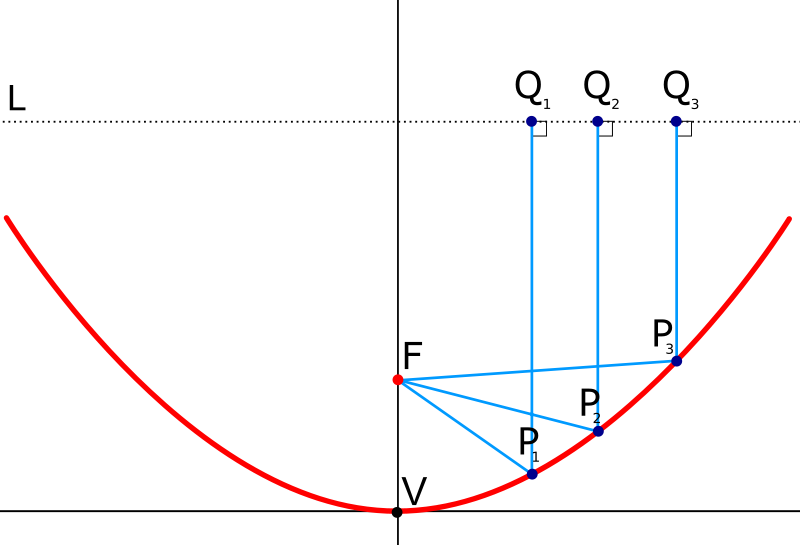
\includegraphics[width=0.4\textwidth-\fboxrule-\fboxrule]{imgs/parabola.png}}  
\end{wrapfigure}

\textbf{Antena isotrópica:} caso ideal, radia potencia  de igual forma en todas las direcciones (\textit{omnidireccional}).

\subsubsection{La antena parabólica de reflexión}

\begin{description}
\item \textbf{Parábola:} lugar geométrico de todos los puntos que equidistan de una línea recta dada (\textit{generatriz}) y de un punto fijo (\textit{foco}) que no pertenecen a la recta.
\end{description}

Las superficies \textit{paraboloides} (parábola de revolución) se usan en las antenas ya que verifica la siguiente propiedad: las ondas reflejadas en una parábola y que provengan de cualquier fuente de energía electromagnética que esté situada en su foco seguirán trayectorias paralelas al eje de la parábola. 

En la práctica hay dispersión debido a que la fuente de energía no se ubica en un punto. Cuanto mayor sea el diámetro de la antena, más direccional será el haz. En el receptor, si las ondas recibidas son paralelas al eje de la parábola reflectante, la señal resultante estará en concentrada en el foco.

Se utiliza en aplicaciones microondas terrestres y satélites.

\subsubsection{Ganancia de una antena}

Es una medida de su \textbf{direccionalidad} (no de potencia), medida en decibelios. Dada una dirección, se define la ganancia como la potencia de salida en esa dirección, comparada con la potencia transmitida en cualquier dirección por una antena isotrópica. El incremento de potencia radiada en una dirección dada se consigue a expensas de la potencia radiada en otras direcciones.

El \textbf{área efectiva} de una antena está relacionada con su tamaño físico y con su geometría, y está dada por:
\[G = \frac{4 \, \pi \, A_e}{\lambda^2} = \frac{4 \, \pi \, f^2 \, A_e}{c^2},\]
donde $G$ es la ganancia, $A_e$ el área efectiva, $\lambda$ la longitud de la portadora, $f$ la frecuencia de la portadora y $c$ la velocidad de la luz.

\subsection{Microondas terrestres}

Antena parabólica tipo <<plato>>, típicamente de 3 metros de diámetro. Se fija rígidamente de forma tal que el haz debe estar perfectamente enfocado siguiendo la trayectoria visual hacia la antena receptora. Se sitúan a alta distancia para disminuir obstáculos en la transmisión, y se interconectan entre varias para alcanzar grandes distancias.

Se usan como alternativas a los métodos de transmisión guiados. Es frecuente su uso en TV y telefonía.

\subsubsection{Características de transmisión}

Cubre la banda de frecuencias de la microondas. Cuanto mayor sea la frecuencia utilizada, mayor es el ancho de banda potencial, y por tanto, mayor es la posible velocidad de transmisión.

La principal causa de pérdidas es la atenuación:
\[L=10 \log \left(\frac{4\,\pi\,d}{\lambda}\right)^2 \text{dB},\]
donde $d$ es la distancia. Al variar al cuadrado (y no exponencialmente, como en los medios guiados), la distancia entre repetidores/amplificadores puede ser mayor. La atenuación aumenta con la lluvia (especialmente, en frecuencias $>10$ GHz) y con las interferencias, por lo que por esto último se regula la asignación de bandas de forma estricta:

\begin{center}
\begin{tabular}{rl}
Larga distancia & 4 GHz a 6 GHz \\ [1ex]
TV por cable & $\approx$ 12 GHz \\ [1ex] 
Punto a punto entre edificios cercanos & $\approx$ 22 GHz \\ [1ex]
\end{tabular}
\end{center}

\subsection{Microondas por satélite}

\begin{description}
\item \textbf{Satélite de comunicaciones:} estación que retransmite microondas. Enlaza dos o más receptores/transmisores terrestres, denominados estaciones base. Recibe una señal en una banda de frecuencia (canal \textit{ascendente}), la amplifica/repite, y la retransmite en otra banda de frecuencia (canal \textit{descendente}). Las bandas de frecuencias se denominan \textbf{canales \textit{transpondedores}}. Para mantenerse constantemente alineado con las estaciones base, el satélite debe estar en una órbita geoestacionaria (35.863 km).
\end{description}

Sus aplicaciones principales están en la difusión de televisión, telefonía a larga distancia y redes privadas.

El rango de frecuencias óptimo va de 1 a 10 GHz. Por debajo de 1 GHz, el ruido producido por causas naturales e interferencias con otros dispositivos electrónicos es apreciable. Por encima de los 10 GHz, existe atenuación por la atmósfera y por las precipitaciones.
\begin{figure}[ht!]
  \caption{Configuraciones de comunicaciones satelitales.}  
  \label{fig:satelite}
  \centering
  \hbox{
   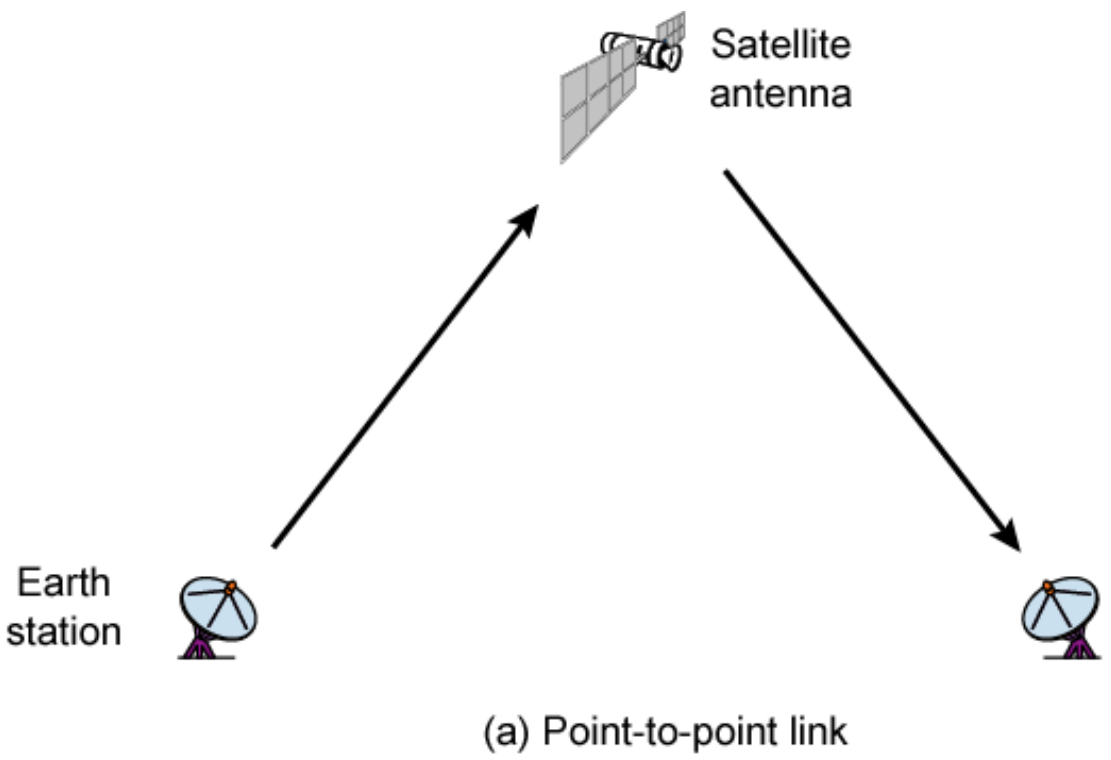
\includegraphics[width=0.44\textwidth-\fboxrule-\fboxrule]{imgs/sat_point_to_point.png}
  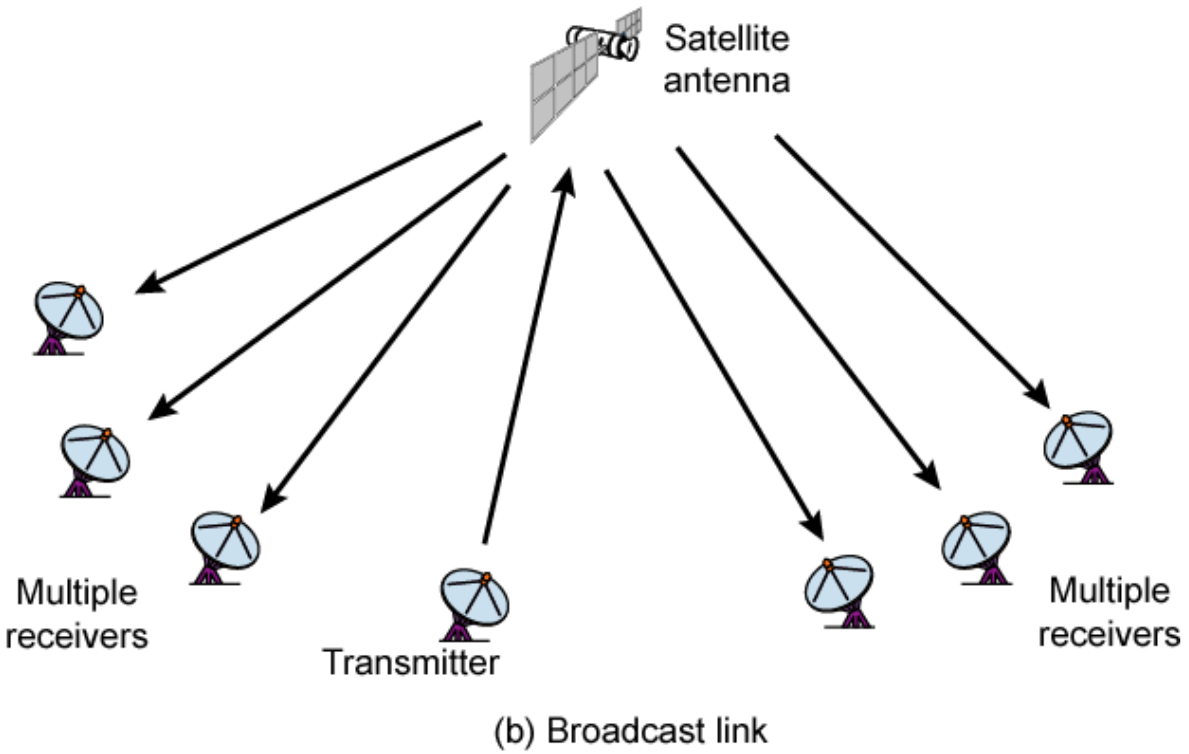
\includegraphics[width=0.5\textwidth-\fboxrule-\fboxrule]{imgs/sat_broadcast.png}}
\end{figure}

La mayoría de los satélites que proporcionan servicio de enlace punto a punto operan en la \textit{banda 4/6 GHz}:
\[
  \textbf{Banda 4/6 GHz} = \left\{ 
  \begin{array}{l l}
    \text{Canal ascendente:} & \text{5.925 a 6.425 GHz}\\
    \text{Canal descendente:} & \text{3.7 a 4.2 GHz}\\
  \end{array} \right.
\]
En una transmisión continua y sin interferencias, no se puede transmitir y recibir en el mismo rango de frecuencias. Por eso es necesario usar bandas de frecuencias distintas.

Debido a las grandes distancias involucradas, se produce un retardo de propagación del orden de un cuarto de segundo.

\begin{multicols}{2}

\subsection{Ondas de radio}

\begin{itemize}
\item Son omnidireccionales. No necesitan antenas parabólicas.
\item Adecuado a la difusión simultánea a varios destinos.
\item Menos sensibles a la atenuación por lluvia.
\end{itemize}
\vfill

\subsection{Infrarrojos}

\begin{itemize}
\item Comunicación mediante transmisores/receptores que modulan luz infrarroja no coherente, que deben estar alineados directamente.
\item No pueden atravesar paredes, por lo que es más seguro y menos susceptible a interferencias.
\item No hay regulación al respecto.
\end{itemize}
\end{multicols}

\section{Propagación inalámbrica}

Toda señal radiada por una antena puede seguir tres posibles trayectorias: la superficial (GW, \textit{ground wave}), la aérea (SW, \textit{sky wave}) o la visual (LOS, \textit{line of sight}).

\begin{figure}[ht!]
  \caption{Distintos tipos de propagación inalámbrica.}  
  \label{fig:gwsw}
  \centering
  \hbox{
   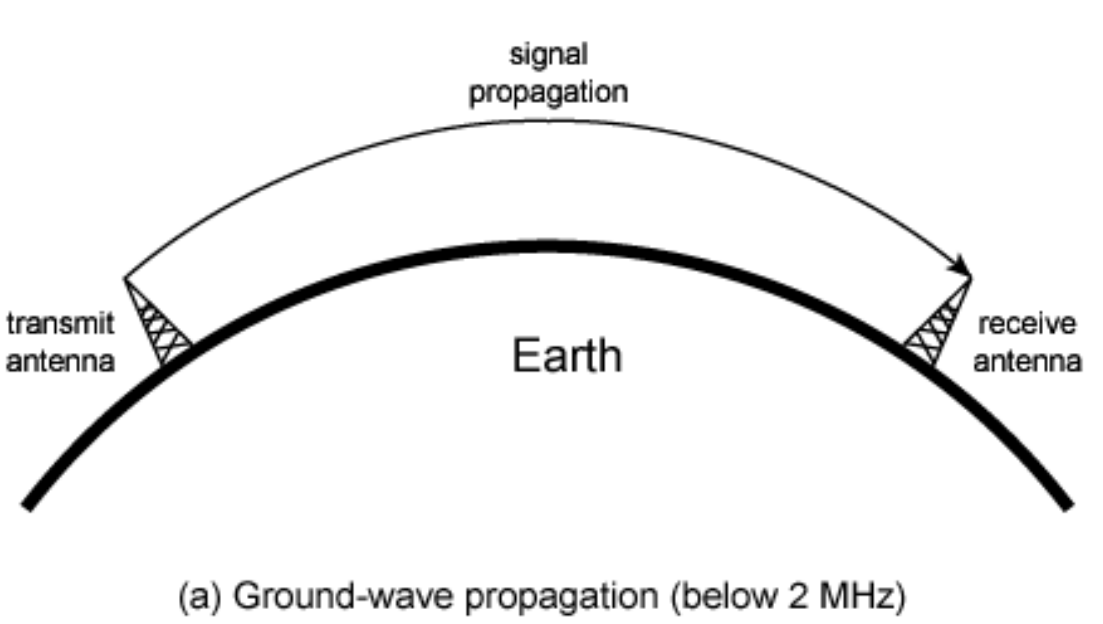
\includegraphics[width=0.5\textwidth-\fboxrule-\fboxrule]{imgs/gw.png}
  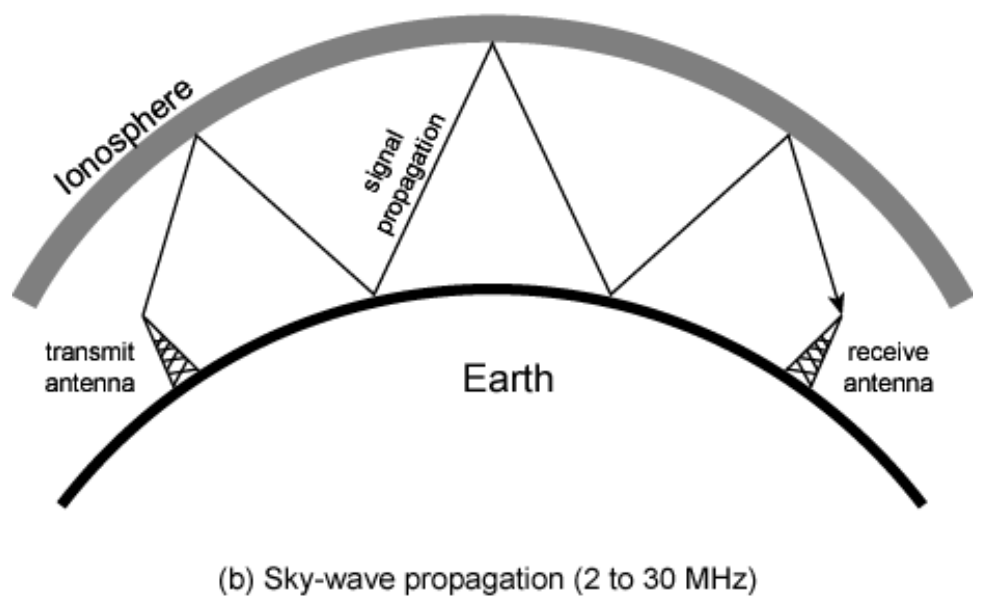
\includegraphics[width=0.5\textwidth-\fboxrule-\fboxrule]{imgs/sw.png}
  } 
  \vspace{0.7cm}
  \centerline{\hbox{
  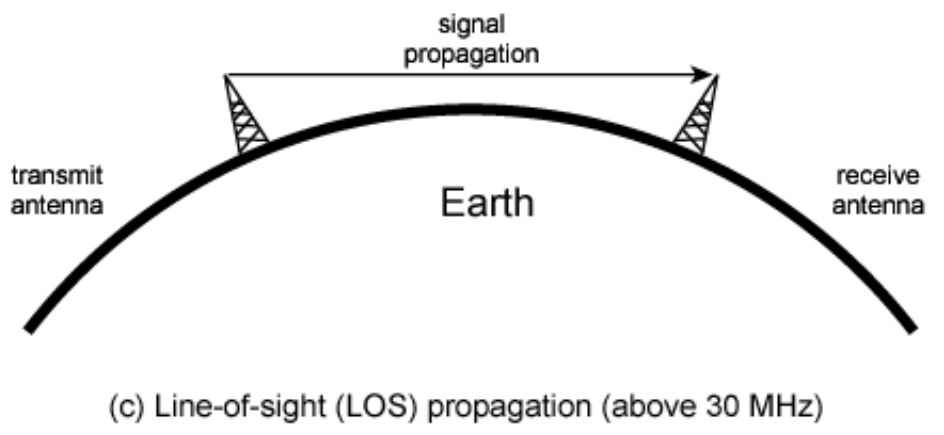
\includegraphics[width=0.5\textwidth-\fboxrule-\fboxrule]{imgs/los.png}  
  }}
\end{figure}

\subsection{Propagación superficial de ondas (GW)}

Sigue el contorno de la superficie terrestre, alcanzando grandes distancias. Este efecto se da hasta 2 MHz. Hay varios factores para que esto ocurra: la onda electromagnética induce una corriente en la superficie terrestre, provocando que la señal se curve; además, sucede un efecto de difracción que ayuda a la curvatura.

\subsection{Propagación área de ondas (SW)}

La señal proveniente de la antena terrestre se refleja en la capa ionizada de la atmósfera alta, volviendo así hacia la tierra. La señal se propaga entonces dando saltos. Es usado por los radio-aficionados.

\subsection{Propagación en la trayectoria visual (LOS)}

Por encima de 30 MHz, el modo SW no funciona. Para este modo de transmisión, la antena emisora y la receptora deben estar alineadas según la trayectoria visual \textit{efectiva} (las microondas son refractadas por la atmósfera). Por lo general, las microondas siguen la curvatura de la tierra, por lo que llegarán más lejos que si siguieran la línea de visión óptica (Figura \ref{fig:optical}).

\begin{wrapfigure}{r}{0.5\textwidth}
  \caption{Horizonte óptico y de radio}
  \label{fig:optical}  
  \centering
  \hbox{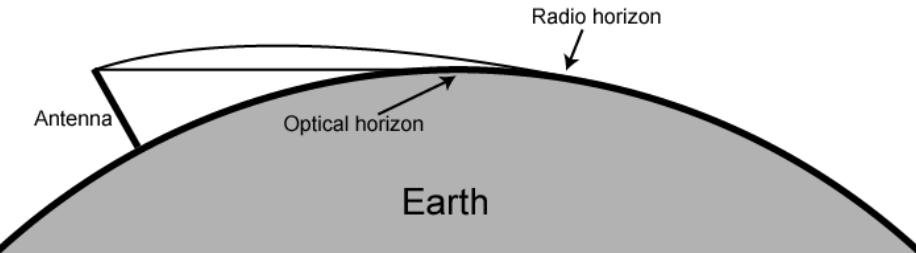
\includegraphics[width=0.5\textwidth-\fboxrule-\fboxrule]{imgs/optical.png}}  
\end{wrapfigure}

\begin{description}
\item \textbf{Refracción:} la onda se desvía hacia el medio más denso. El \textbf{índice de refracción} de la atmósfera disminuye con la altura, por ello las ondas viajarán más rápido mientras más alejadas estén de la tierra.
\end{description}

\subsection{Línea de visión óptica y efectiva}

Si no hay obstáculos, la \textbf{línea de visión óptica} se puede expresar cómo:
\[d=3.57 \, \sqrt{h},\]
donde $d$ es la distancia entre la antena y el horizonte en kilómetros, y $h$ es la altura en metros.

La \textbf{línea de visión efectiva} se expresa como:
\[d=3.57 \, \sqrt{Kh},\]
donde $K$ es un factor de ajuste por refracción ($K \approx 4/3$).

La distancia máxima entre dos antenas de altura $h1$ y $h2$ está dada entonces por:
\[d=3.57 \, (\sqrt{Kh_1} + \sqrt{Kh_2}).\]

\subsection{Transmisión en la trayectoria visual}

Cualquier comunicación inalámbrica se dispersa con la distancia, siendo esta la causa principal de las pérdidas en las comunicaciones satelitales. Incluso si no hubiera ruido, al aumentar la distancia, la señal se atenúa ya que va aumentando su área ocupada. Esta atenuación se denomina \textbf{pérdida en el espacio libre} y se calcula como:
\[ \frac{P_e}{P_r} =  \frac{(4\pi d)^2}{\lambda^2} = \frac{(4\pi f d)^2}{c^2} = \frac{(c\,d)^2}{f^2 \,A_{r}\,A_{e}}, \]
donde el sufijo $e$ denota antena emisora y $r$ receptora, $d$ la separación entre las antenas, $c$ la velocidad de la luz, $\lambda$ la longitud de onda de la portadora, y $A$ las áreas efectivas de las antenas.

Se puede reescribir la ecuación de pérdida como:
\[L_{\text{dB}} = 20 \log(f) + 20\log(d) - 10 \log(A_r A_e) + 169.54 \text{dB},\]
por tanto, cuanto mayor $\lambda$, mayor pérdida. Así también, a más altas frecuencias, menos pérdidas.

\subsection{Multitrayectorias}

La señal se refleja en tantos obstáculos que llegan varias versiones de la misma señal con retardos diferentes.

\subsection{Pérdidas de desvanecimiento}

\begin{figure}[ht!]
  \caption{Tabla de pérdidas por desvanecimiento. La fórmula resultante de la \textbf{pérdida por desvanecimiento} $L_d$ en decibelios está dada por la suma de cada uno de los términos de la primera columna. }  
  \label{fig:desvanecimiento}
  \centering
  \hbox{
   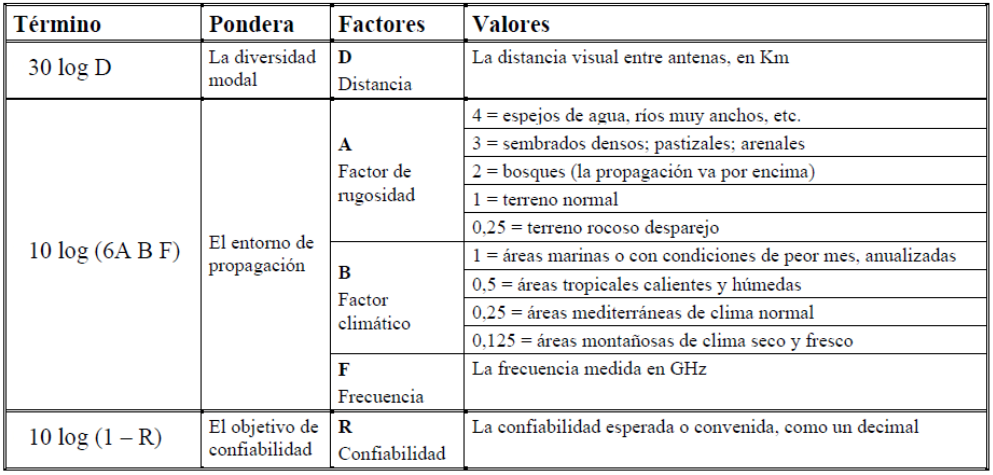
\includegraphics[width=\textwidth-\fboxrule-\fboxrule]{imgs/desvanecimiento.png}}
\end{figure}

\pagebreak

\section{La Capa de Enlace de Datos (CED)}

Provee los algoritmos para lograr una comunicación confiable y eficiente entre dos máquinas adyacentes\footnote{Dos máquinas conectadas por un canal de comunicaciones que actúa de manera conceptual como un alambre, es decir, los bits se reciben en el mismo orden en el que son enviados.}.

Existe una serie de problemas y limitaciones al sólo hecho de transmitir bits:
\begin{itemize}
\item Hay errores ocasionales.
\item La tasa de datos es finita.
\item Hay retardo de propagación.
\end{itemize}

\subsection{Cuestiones de diseño}

La capa debe desempañar varias funciones específicas, incluidas:
\begin{enumerate}
\item Proporcionar una interfaz de servicio bien definida con la capa de red.
\item Manejar los errores de transmisión.
\item Regular el flujo de datos para evitar saturar receptores lentos.
\item \textbf{Primordial}: el armado y manejo de \textbf{tramas}\footnote{La capa de enlace de datos toma de la capa de red los paquetes y los encapsula en tramas.}.
\end{enumerate}

\begin{figure}[ht!]
  \caption{Relación entre los paquetes y las tramas.}
  \label{fig:paquetes_tramas}
  \centerline{\hbox{
   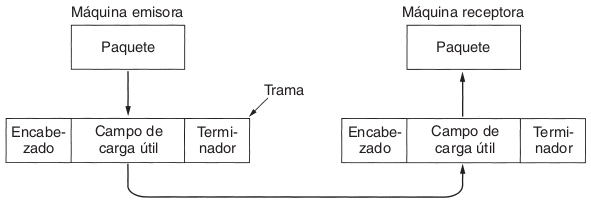
\includegraphics[width=0.7\textwidth-\fboxrule-\fboxrule]{imgs/paquetes_tramas.png}}}
\end{figure}

\subsubsection{Servicios proporcionados a la capa de red (CdR)}

El principal es el de transferir los datos de la CdR en la máquina origen a la CdR de la máquina destino.

La CED puede diseñarse para ofrecer varios tipos de servicios:
\begin{description}
\item \textbf{Servicio no orientado a la conexión sin confirmación de recepción.} Consiste en hacer que el origen envíe tramas independientes al destino sin pedir que éste confirme la recepción. Si una trama se pierde, la CED no hace ningún intento por detectar la pérdida y recuperarse de ella. Es apropiado cuando el BER (\textit{bit error rate}) es bajo, o cuando el tráfico es en tiempo en real (telefonía).
\item \textbf{Servicio no orientado a la conexión con confirmación de recepción.} Se confirma de manera individual la recepción de cada trama enviada. De esta manera, el emisor sabe si la trama ha llegado bien o no. Si no ha llegado en un tiempo específico, puede reenviarse. Es útil en canales inestables (sistemas inalámbricos).
\item \textbf{Servicio orientado a la conexión con confirmación de recepción.} El origen y destino establecen una conexión antes de transferir datos. Cada trama enviada estará enumerada, y la CED garantizará que cada trama llegue a su destino, una sola vez y en el orden adecuado. Aquí, las transferencias tendrán tres fases distintas:
\begin{enumerate}
\item Establecer conexión, inicializando en ambos lados variables y contadores.
\item Transmitir una o más ramas.
\item Cerrar conexión y liberar recursos.
\end{enumerate}
\end{description}

\underline{Nota}: proporcionar confirmaciones de recepción en la CED sólo es una optimización, no un requisito.

\subsubsection{Entramado}
La capa física acepta un flujo de bits puros e intenta entregarlo al destino, sin garantizar ausencia de errores. La CED debe ser capaz detectar y corregir los errores. Para ello, divide el flujo de bits en tramas separadas, calcula la \textbf{suma de verificación} (\textit{checksum}) de cada una, y se las adjunta. Al llegar a destino, se recalcula el \textit{checksum} y, si es distinto al contenido en la trama, se sabe que hubo un error y se toman medidas para arreglarlo.

Para la división en tramas del flujo de bits, se necesita una forma de detectar el inicio y fin de cada trama. Para evitar depender de la temporización (que es riesgoso a causa de demoras imprevistas), se han creado otros métodos:
\begin{description}
\item \textbf{Conteo de caracteres.} El entramado contiene un campo en el encabezado para especificar el número de caracteres en la trama. La CED de destino ve la cuenta de caracteres y sabe entonces donde está el fin de la trama.
\subitem \textit{Problema:} la cuenta puede alterarse por un error de transmisión, por lo que no hay forma de saber donde termina y donde comienza la otra trama.
\item \textbf{Banderas con relleno de caracteres.} Evita el problema de tener que resincronizar luego de un error, haciendo que cada trama inicie y termine con bytes especiales. Generalmente son la misma, por lo que dos banderas seguidas señalan el inicio y fin de una trama.
Se puede dar con facilidad un \textit{payload}\footnote{Al trabajar con datos binarios, el patrón de bits que aparece en los datos a transmitir puede coincidir con el de una bandera.} Para evitarlo, se inserta un byte de escape especial justo antes de cada bandera en los datos, y es removido en el destino por la CED. Si además aparece el símbolo de escape en los datos, también se le aplica el mismo procedimiento.
\subitem \textit{Problema:} Está fuertemente atada a caracteres de 8 bits. No funciona con tamaños arbitrarios.
\item \textbf{Banderas de inicio y fin, con relleno de bits.} Solventa el problema del método anterior, al utilizar bits en vez de caracteres. Cada trama comienza y termina con una bandera (01111110). Si encuentra cinco bits 1 consecutivos en los datos, le inserta un bit 0 al final, que se remueve al llegar al destino por la CED (para evitar banderas en los datos).
\item \textbf{Violaciones de codificación en la capa física.} Sólo se aplica cuando la codificación contiene redundancia (transición a mitad del intervalo). Las violaciones del código (bajo$\rightarrow$bajo ó alto$\rightarrow$alto) delimitan la trama.
\end{description}

\subsubsection{Control de Errores}

Se plantea el problema: ¿Cómo asegurar que todas las tramas realmente se entreguen en el orden apropiado? Para resolverlo, se pueden ir implementando las siguientes opciones:
\begin{itemize}
\item Exigir al receptor que regrese tramas de control especiales que confirmen la recepción o no de cada trama.
\item Implementar temporizadores de espera de confirmación de recepción, que al expirar reenvíen la trama ``fallida''. El intervalo de espera debe ser lo suficientemente grande para esperar la ida y vuelta de las trama.
\item Asignar números de secuencias a las tramas enviadas para evitar que el receptor acepte la misma trama múltiples veces.
\end{itemize}

\subsubsection{Control de Flujo}

¿Qué hacer cuando el receptor recibe más tramas de las que puede aceptar a causa de un emisor rápido?

Para evitar que el receptor pierda las tramas que recibe, se utilizan dos métodos:
\begin{description}
\item \textbf{Control de flujo basado en retroalimentación.} El receptor regresa información al emisor autorizándolo para enviar más datos o indicándole su estado.
\item \textbf{Control de flujo basado en tasa.} Se limita la tasa a la que el emisor envía datos, sin recurrir a la retroalimentación por parte del receptor (no se utiliza en la CED).
\end{description}

\subsection{Detección y corrección de errores}

Hay dos maneras de lidiar con los errores: \textbf{detectarlos solamente}, o \textbf{detectarlos y corregirlos.}

Si la transmisión es altamente confiable (\textit{fibra óptica}), es más económico retransmitir los bloques defectuosos que surgen ocasionalmente. En caso de que haya muchos errores (\textit{transmisión inalámbrica}), es mejor agregar suficiente redundancia para corregirlos.

%%%% QUEDA PENDIENTE

\subsection{Protocolos elementales de enlace de datos}

Antes de estudiar los protocolos, se harán una serie de suposiciones:
\begin{itemize}
\item Las capas física, de enlace, y de red contienen procesos independientes.
\item La máquina $A$ envía flujos de datos a $B$.
\item Se usa el servicio confiable orientado a la conexión.
\item $A$ tiene un suministro infinito de datos listos para ser enviados.
\item Las máquinas no fallan.
\item Los paquetes transmitidos de la CR a la CED contienen datos puros.
\item La trama contiene información de control (encabezado), un paquete, y un \textit{checksum} (terminador).
\item La CF recibe una trama, calcula su \textit{checksum}. Si no está dañada, revisa el encabezado y luego le pasa el paquete a la CR, sin el dicho encabezado ni el terminador.
\item El canal es inestable y pierde tramas completas ocasionalmente.
\item Se usa un temporizador en el emisor.
\end{itemize}

\subsubsection{Protocolo simplex sin restricciones}

Los datos se transmiten solo en una dirección; las capas de red siempre están listas; se ignora el tiempo de procesamiento; espacio infinito de búfer; el canal nunca tiene problemas ni pierde tramas; el emisor está en un ciclo infinito que sólo envía tramas.

\subsubsection{Protocolo simplex de parada y espera}

Ahora la CED no tiene un espacio infinito de búfer. Entonces, se debe evitar que el emisor sature al receptor: se soluciona haciendo que el receptor retroalimente al receptor, enviándole una señal de confirmación de recepción para transmitir la próxima trama (\textbf{parada y espera}).

Las tramas viajan en ambas direcciones: se necesitaría un canal físico semiduplex.

\subsubsection{Protocolo simplex para un canal con ruido}

Ahora se comenten errores en el canal: las tramas pueden salir dañadas o perderse. Pero suponemos que si se dañó, podremos detectarlo al calcular el \textit{checksum}.

Se agrega un temporizador para esperar por la trama de confirmación (que puede perderse).

Para evitar aceptar tramas duplicadas, se les agrega un número de secuencia de 1 bit (0 ó 1). El receptor espera un número de secuencia en particular, y si cuando llega una trama esta tiene el número correcto, se acepta y se envía a la CR. A continuación, el número de secuencia se invierte, y se avisa de esto al emisor para que envíe otra trama (\textbf{PAR, \textit{confirmación de recepción positiva con retrotransmisión}}).

\subsection{Protocolos de ventana corrediza}

En la mayoría de las aplicaciones se necesitan transmitir datos en ambas direcciones. Se mezclan las tramas de confirmación de recepción con la de datos. Analizando el encabezado se puede distinguir si es una u otra.

\begin{description}
\item \textbf{Piggybacking.} Cuando llega una trama de datos, el receptor aguanta y espera un lapso fijo de tiempo hasta que la CR le pasa el siguiente paquete, y entonces la confirmación de recepción se anexa al tramo de datos de salida (viajando gratuitamente). Esto mejora el uso del ancho de banda y los tiempos de procesamiento.

Pero, si dado un cierto lapso de tiempo no llega ningún nuevo paquete, la CED envía una trama de confirmación de recepción independiente.
%
\item \textbf{Ventana corrediza.} Clase de protocolos bidireccionales. Cada trama de salida contiene un número de secuencia de 0 a $2^n-1$, para un campo de $n$ bits. Posee dos tipos de ventanas (que no necesitan poseer el mismo tamaño):
\begin{itemize}
\item \textbf{Ventana emisora:} en cualquier instante, el emisor mantiene un grupo de números de secuencia que corresponde a las tramas que tiene permitido enviar. Dados que estas pueden perderse o dañarse, el emisor debe mantener todas estas tramas en su memoria para su posible retransmisión (necesita $n$ búferes).
\item \textbf{Ventana receptora:} de manera similar, en el receptor se mantiene el grupo de tramas que tiene permitido aceptar. Al recibir un trama, si no está en la ventana, es descartada; de lo contrario, se envía a la CR, se genera una confirmación de recepción y se incrementa la ventana en uno.
\end{itemize}
\end{description}

\begin{figure}[ht!]
  \caption{Ventana corrediza de tamaño 1, con un número de secuencia de 3 bits. (a) Al inicio. (b) Tras la transmisión de la primera trama. (c) Tras la recepción de la primera trama. (d) Tras recibir la primera confirmación de recepción.}
  \label{fig:ventana_corrediza}
  \centerline{\hbox{
   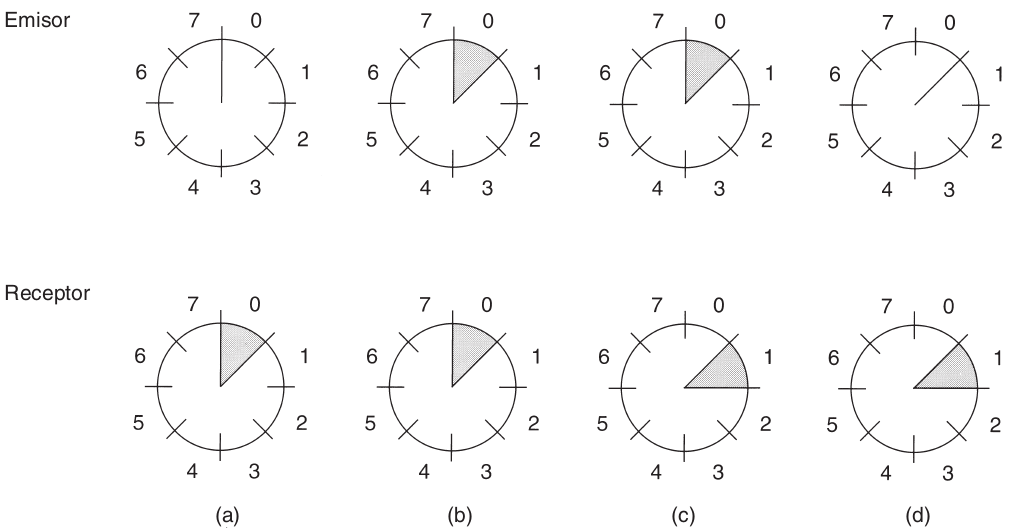
\includegraphics[width=0.85\textwidth-\fboxrule-\fboxrule]{imgs/ventana_corrediza.png}}}
\end{figure}

\subsubsection{Ventana corrediza de un bit}

Utiliza parada y espera, con un $n=1$.

\subsubsection{Protocolo que usa retroceso N}

Si el tiempo necesario para que una trama llegue al receptor más el necesario para que la confirmación de recepción regrese no es despreciable, nos enfrentamos a un problema.

La solución está en la \textbf{canalización}, o sea, permitir que el emisor envíe hasta $w$ tramas antes de bloquearse, en lugar de 1. Si el producto del \textbf{ancho de banda} por el \textbf{retardo del viaje de ida y vuelta} es grande, la ventana en el lado emisor debe ser grande. Estos dos factores indican cual es la capacidad del canal, y el emisor necesita la capacidad de llenarlo sin detenerse para funcionar eficazmente.

\begin{figure}[ht!]
  \caption{Canalización y recuperación de un error. Efecto del error cuando $n=1$ (a), y cuando $n=$grande (b).}
  \label{fig:canalizacion}
  \centerline{\hbox{
   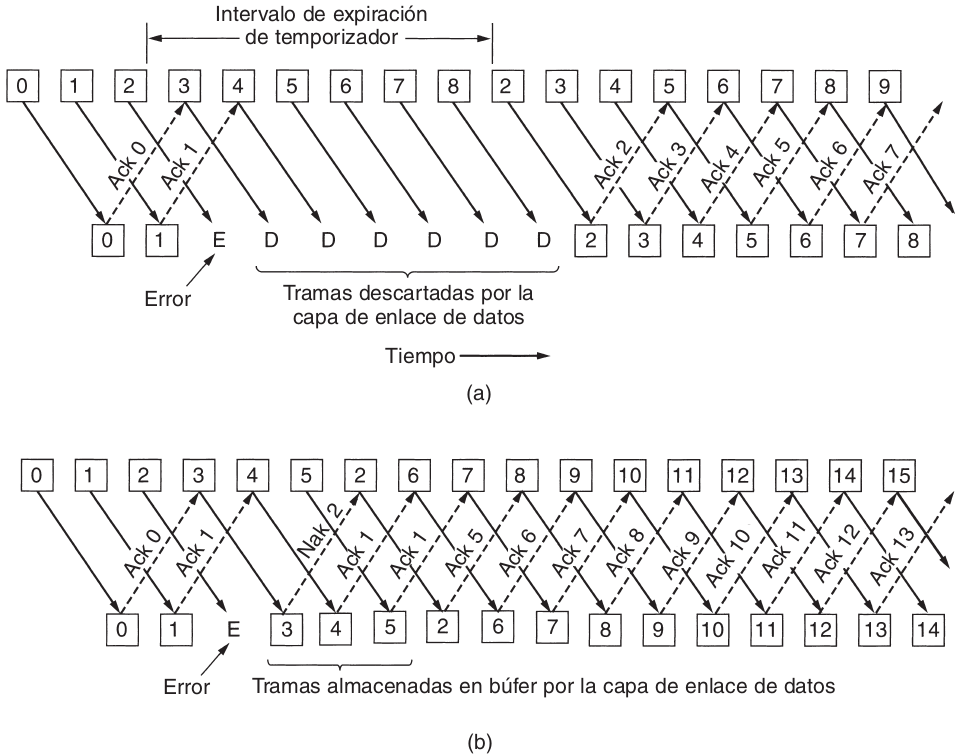
\includegraphics[width=0.85\textwidth-\fboxrule-\fboxrule]{imgs/canalizacion.png}}}
\end{figure}

Hay dos métodos básicos para manejar errores durante la canalización:
\begin{description}
\item \textbf{Retroceso n:} el receptor descarta todas las tramas subsecuentes, sin enviar confirmación de recepción (\textit{ACK}), hasta que le llega la que esperaba. Usa ventana con $n=1$. Esta estrategia puede desperdiciar bastante ancho de banda si la BER es alta.
\item \textbf{Repetición selectiva:} se descarta una trama dañada recibida, pero las tramas en buen estado recibidas después de ésa se almacenan en un búfer. Cuando el emisor termina, sólo la última trama sin confirmación se retransmite. Si la trama llega correctamente, el receptor puede entregar a la CR, en secuencia, todas las tramas que ha almacenado en el búfer. Se debe agregar un temporizador por cada trama pendiente en el emisor. La retransmisión de una trama específica puede ser acelerada incluyendo una confirmación de recepción negativa (\textit{NAK}) que avise que no se recibió esa trama correctamente, evitando esperar a que expire el temporizador asociado. 
\subitem La recepción no secuencial introduce cierto problema: una vez que el receptor ha avanzado su ventana, el nuevo intervalo de números de secuencia válidos se traslapa con el anterior, por lo que podría haber tramas duplicadas. Para evitar esto, el tamaño de la ventana debe ser como máximo la mitad a la cantidad los números de secuencia. Ejemplo:
\[\text{4 bits para números de secuencia} \Rightarrow 16 \text{ números } \neq \Rightarrow \text{ventana de tamaño máximo 8 } [0,..,7].\]
\subitem La cantidad de búferes y temporizadores asociados necesarios es igual al tamaño de la ventana.
\end{description}

\underline{Nota:} La primera estrategia se enfoca en el ancho de banda, y la segunda en el tamaño del búfer. Dependiendo de que recurso sea más valioso, se usará una u otra.

\subsection{Ejemplos de protocolos de Enlace de Datos}

\subsubsection{HDLC - Control de Enlace de Datos de Alto Nivel}

Es orientado a bits y usa relleno de bits para lograr la transparencia de los datos.

\begin{figure}[ht!]
  \caption{Formato de trama para protocolos orientados a bits.}
  \label{fig:hdlc}
  \centerline{\hbox{
   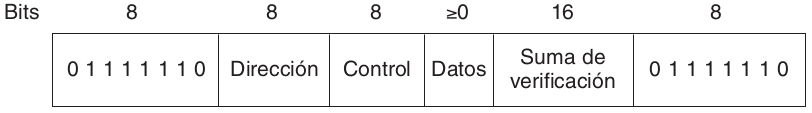
\includegraphics[width=0.7\textwidth-\fboxrule-\fboxrule]{imgs/hdlc.png}}}
\end{figure}

Posee los siguientes campos (ver Figura \ref{fig:hdlc}):
\begin{description}
\item \textbf{Dirección.} Sirve para identificar cada terminal en múltiples terminales. A veces se usa para distinguir los comandos de las respuestas.
\item \textbf{Control.} Se utiliza para números de secuencias, ACK, y otros propósitos.
\item \textbf{Datos.} Contiene cualquier información y es de longitud variable.
\item \textbf{Checksum.} Código de redundancia cíclica.
\end{description}
La trama está delimitada por otra secuencia de bandera (01111110).

\begin{figure}[ht!]
  \caption{Campo de \textit{Control} de una trama (a) de información, (b) de supervisión, y (c) no numerada.}
  \label{fig:tipo_trama}
  \centerline{\hbox{
   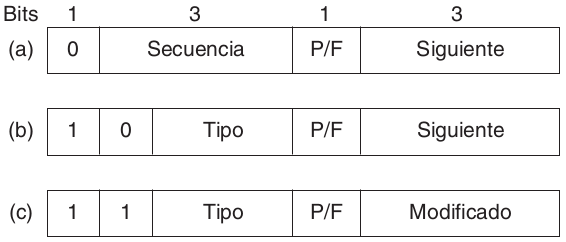
\includegraphics[width=0.5\textwidth-\fboxrule-\fboxrule]{imgs/tipo_trama.png}}}
\end{figure}

Hay tres tipos de tramas, que difieren entre sí en la información del campo de \textit{control}. Estas son:
\begin{enumerate}
\item \textbf{Información.}
\begin{itemize}
\item \textit{Secuencia.} Número de secuencia de la trama.
\item \textit{Poll/Final (P/F).} Cuando se indica $P$, se invita a la terminal a enviar datos. Cuando se usa $F$, se marca el final de envío de datos.
\item \textit{Siguiente.} Confirmación de ACK superpuesta (cuál es la siguiente trama esperada).
\end{itemize}
\item \textbf{Supervisión.} Las distintas tramas poseen diferentes valores en el campo \textit{Tipo}:
\begin{itemize}
\item \textit{RECEIVE READY (Tipo 0):} se utiliza como ACK cuando no hay superposición.
\item \textit{REJECT (Tipo 1):} indica que se ha detectado un error. Se pide al receptor retransmitir todas las tramas desde la indicada en el campo \textit{Siguiente} en adelante.
\item \textit{RECEIVE NOT READY (Tipo 2):} las tramas enviadas han sido aceptadas, pero indica que se detenga el envío. Señala problemas temporales en el receptor.
\item \textit{SELECTIVE REJECT (Tipo 3):} como REJECT, pero pide sólo la retransmisión de la trama específicada.
\end{itemize}
\item \textbf{No numerada.} Se usa para el control pero también para llevar datos cuando se usa un \textit{servicio no confiable}. Varía mucho entre los distintos protocolos.
\end{enumerate}

\subsubsection{PPP - Protocolo Punto a Punto}

Realiza detección de errores, soporta múltiples protocolos, permite la negociación de direcciones de IP en el momento de la conexión, permite la autenticación y tiene muchas otras funciones. Está orientado a bits y usa relleno de bytes, por lo que todas las tramas tienen un número entero de bytes.

Proporciona además tres características:
\begin{enumerate}
\item Entramado sin ambigüedades en el final y el inicio. El formato de trama también maneja detección de errores.
\item \textbf{Protocolo de Control de Enlace} (LCP), para activar líneas, probarlas, negociar opciones y desactivarlas ordenadamente.
\item \textbf{Protocolo de Control de Red} (NCP), para negociar opciones de CR con independencia del protocolo de red usado.
\end{enumerate}

\begin{figure}[ht!]
  \caption{Formato de trama completa PPP para el modo de operación no numerado. El tamaño de la \textit{carga útil} por \textit{default} es de 1500 bytes, con relleno si es necesario.}
  \label{fig:ppp}
  \centerline{\hbox{
   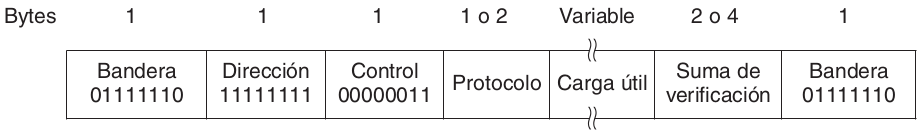
\includegraphics[width=0.75\textwidth-\fboxrule-\fboxrule]{imgs/ppp.png}}}
\end{figure}

PPP soporta detección de errores, negociación de opciones, compresión de encabezados y no proporciona  de manera predeterminada transmisión confiable. Opcionalmente, se puede tener transmisión confiable con formato de tramas similar al de HDLC.

\begin{figure}[ht!]
  \caption{Diagrama de fases simplificado para activar y desactivar una línea. PPP inicia en \textit{Muerta}.}
  \label{fig:ppp_fases}
  \centerline{\hbox{
   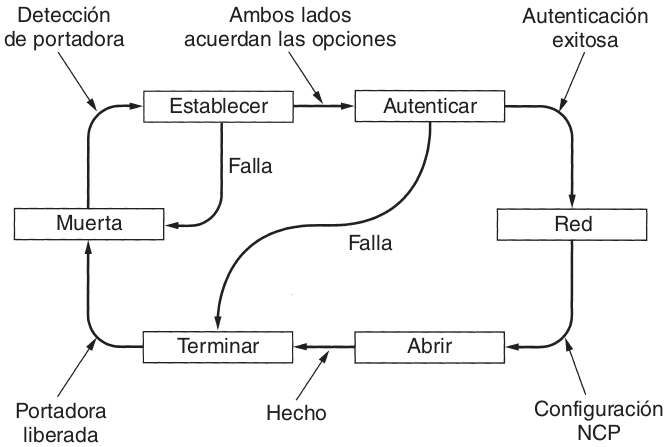
\includegraphics[width=0.57\textwidth-\fboxrule-\fboxrule]{imgs/ppp_fases.png}}}
\end{figure}

\pagebreak
\section{La Subcapa de Control de Acceso al Medio (MAC)}

Esta sección es sobre las redes que usan difusión y sus protocolos. En cualquier red de difusión el asunto clave es la manera de determinar quién puede utilizar el canal cuando hay competencia por él. Los protocolos usados para determinar esto pertenecen a una subcapa inferior de la CED llamada subcapa de \textbf{Control de Acceso al Medio} (\textbf{MAC}).

La MAC se encarga de la topología lógica de la red y del método de acceso a ésta. Cada tecnología de red tiene una subcapa MAC diferente. Además, aquí residen las direcciones MAC.

\subsection{El problema de asignación del canal}

\textit{¿Cómo se asigna un solo canal de difusión entre varios usuarios?}

\subsubsection{Asignación estática de canal en LANs y MANs}

La manera tradicional es usando FDM (\textit{Multiplexación por División en Frecuencia}). Si hay $N$ usuarios, el ancho de banda se divide en $N$ partes de igual tamaño y se le asigna una a cada usuario; de esa forma, no hay interferencia.

El dividir el canal disponible en subcanales estáticos es inherentemente ineficiente. El problema básico es que, cuando algunos usuarios están inactivos, su ancho de banda simplemente se pierde. No lo están usando, y a nadie más se le permite usarlo.

Los mismos argumentos que se aplican a la FDM se aplican a la TDM (\textit{Multiplexación por División de Tiempo}). A cada usuario se le asigna cada N-ésima ranura de tiempo. Si un usuario no usa la ranura asignada, simplemente se desperdicia. Lo mismo se aplica si dividimos las redes físicamente.  Aparte, ninguno de los métodos de asignación estática de canal funciona muy bien con el tráfico en ráfagas, pero tienen sentido cuando existe un número pequeño y constante de usuarios, y cada uno tiene suficientes datos para mantener ocupado el canal.

\subsubsection{Asignación dinámica de canales en LANs y MANs}

Todo el trabajo aquí se basa en cinco supuestos clave, que se describen a continuación.

\begin{enumerate}
\item \textbf{Modelo de estación:} $N$ estaciones \textbf{independientes}, después de generar una trama cada estación se bloquea hasta que su trama es transmitida con éxito. Probabilidad de generar una trama: $\lambda \Delta t$.
\item \textbf{Canal único:} solamente hay un canal para todas las estaciones y todas son equivalentes. 
\item \textbf{Colisiones:} si dos estaciones transmiten simultáneamente hay colisión y las estaciones reconocen las colisiones. La trama colisionada debe retransmitirse después. Son los únicos errores.
\item 
\begin{enumerate}
\item \textbf{Tiempo continuo:} la transmisión puede iniciar en cualquier instante del tiempo, no hay reloj maestro que divida el tiempo en intervalos discretos.
\item \textbf{Tiempo ranurado:} el tiempo se divide en ranuras de tiempo o slots, la transmisión se inicia siempre al inicio del slot.
\end{enumerate}
\item
\begin{enumerate}
\item \textbf{Detección de portadora:} las estaciones no transmiten si el canal está ocupado y pueden detectar esta situación.
\item \textbf{Sin detección de portadora:} las estaciones no pueden detectar el canal antes de intentar usarlo, simplemente transmiten. Sólo después pueden determinar si la transmisión tuvo éxito.
\end{enumerate}
\end{enumerate}

\subsection{Protocolos de acceso múltiple}

\begin{description}
\item \textbf{Colisión:} cuando dos o más tramas son enviadas \textbf{simultáneamente} por el canal único.
\item \textbf{Contienda, Contención, o Competencia:} cuando múltiples sistemas deben tratar de ganar el canal común para su uso irrestricto.
\item \textbf{Persistencia:} la característica de un protocolo de iniciar la
transmisión al encontrar el canal libre después de esperar por él.
\end{description}

\subsubsection{ALOHA}

\begin{description}
\item \textbf{ALOHA puro.} Permite que los usuarios transmitan cuando tengan datos para enviar. Las tramas son transmitidas en tiempos completamente arbitrarios, y \textbf{no se verifica si el canal está ocupado antes de transmitir}. Si se produce una colisión, se espera un tiempo aleatorio y se reenvía. Si no se puede escuchar mientras se transmite, se necesitan ACKs. Uso del canal del 18\%.
\item \textbf{ALOHA ranurado.} Divide el tiempo en intervalos discretos (requiere reloj maestro), cada uno de los cuales corresponde a una trama por vez. Las estaciones únicamente inician la transmisión al principio de cada ranura. Se reducen las colisiones. Hay un aprovechamiento del 36\% del canal.
\end{description}

\begin{figure}[ht!]
  \caption{Velocidad real de transporte contra tráfico ofrecido en los sistemas ALOHA.}
  \label{fig:aloha}
  \centerline{\hbox{
   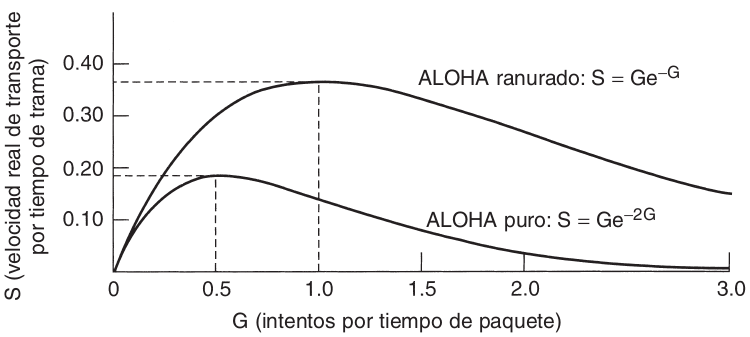
\includegraphics[width=0.65\textwidth-\fboxrule-\fboxrule]{imgs/aloha.png}}}
\end{figure}

\subsubsection{Protocolos de acceso múltiple con detección de portadora}

Escuchan una portadora y deciden que hacer en consecuencia.

\begin{description}
\item \textbf{CSMA (Carrier Sense Multiple Access) persistente y no persistente:}
\begin{itemize}
\item \textbf{\textit{Persistente-1}:} el protocolo inicia la transmisión con una probabilidad 1 cuando encuentra el canal libre después de esperar. Si está ocupado, escucha \textbf{permanentemente} hasta que se libere. Si hay una colisión, espera un tiempo aleatorio y retransmite.
\item \textbf{\textit{No persistente}:} como el anterior, pero no escucha permanentemente, sino que espera un tiempo aleatorio, y vuelve a escuchar.
\item \textbf{\textit{Persistente-$p$}} (para canales \textit{ranurados}): cuando una estación está lista para enviar, escucha el canal. Si éste se encuentra inactivo, la estación transmite con una probabilidad $p$, y con una probabilidad $q = 1 - p$, se espera hasta la siguiente ranura. Si esa ranura también está inactiva, la estación transmite o espera nuevamente, con probabilidades $p$ y $q$ respectivamente. Si está ocupada, espera a la siguiente ranura.
\end{itemize}
\item \textbf{CSMA/CD (Carrier Sense Multiple Access with Collision Detection):} todas las estaciones abortan la transmisión tan pronto detectan la colisión, esperan un tiempo aleatorio, y retransmiten. Se utiliza en Ethernet. 
\subitem El tiempo mínimo para detectar la colisión es sólo el tiempo que tarda la señal para propagarse de una estación a otra ($2\,\tau$). Se modela el intervalo de contienda como un ALOHA ranurado con ancho $2\,\tau$. La colisión debe poder detectarse; por ello la codificación de la señal
debe permitir la detección (no puede haber bits de 0 voltios). El canal debe ser semi-dúplex, debido a que se busca constantemente en busca de colisiones.
\end{description}

\begin{figure}[ht!]
  \caption{Velocidad real de transporte contra tráfico ofrecido en los sistemas ALOHA.}
  \label{fig:comparacion_protocolos}
  \centerline{\hbox{
   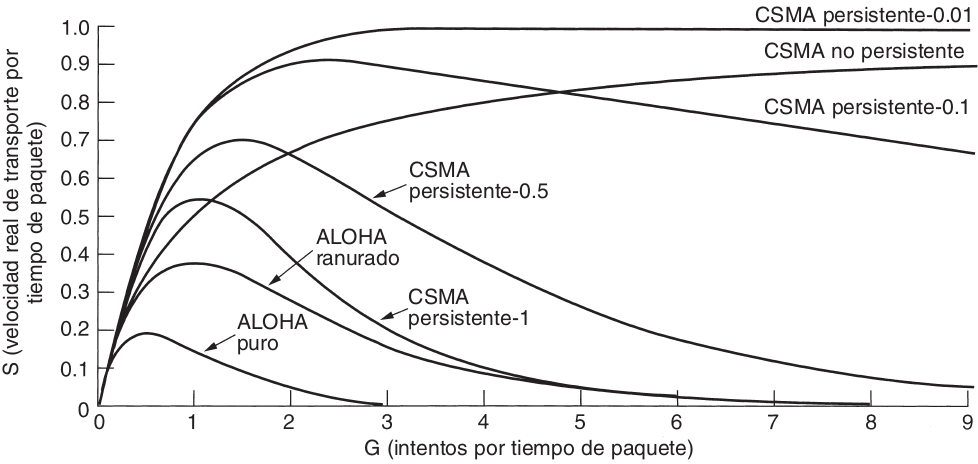
\includegraphics[width=0.85\textwidth-\fboxrule-\fboxrule]{imgs/comparacion_protocolos.png}}}
\end{figure}

\subsubsection{Protocolos libres de colisiones}

Resuelven la contención por el canal sin que haya colisiones, ni siquiera durante el periodo de contención. Suponemos que hay $N$ estaciones, cada una con una dirección única de 0 a $N-1$ incorporada en hardware.

\begin{description}
\item \textbf{Mapa de bits.} Es un protocolo de reservación. Cada periodo de contención consiste en exactamente $N$ ranuras. Si una estación $j$ tiene una trama por enviar, transmite un bit 1 durante la ranura $j$. No está permitido a ninguna otra estación transmitir durante esta ranura. No escala bien para miles de estaciones. Eficiencia a baja carga: $d/(N+d)$, y a carga alta: $d/(d+1)$.

\begin{figure}[ht!]
  \caption{Protocolo básico de mapa de bits.}
  \label{fig:mapa_bits}
  \centerline{\hbox{
   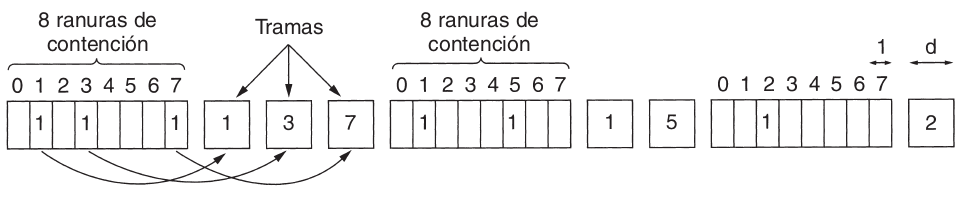
\includegraphics[width=0.85\textwidth-\fboxrule-\fboxrule]{imgs/mapa_bits.png}}}
\end{figure}

\item \textbf{Conteo descendente binario.} Una estación que quiere utilizar el canal ahora difunde su dirección como una cadena binaria de bits, comenzando por el bit de orden mayor. Las direcciones son combinadas con un OR. La estación que encuentra que su 0 fue sobrescrito por un 1 se rinde. 
Las estaciones con números grandes tienen mayor prioridad (que puede ser bueno o malo, según contexto).
Su eficiencia es de $d/(d+\log_2 N)$.
\end{description}

\begin{figure}[ht!]
  \caption{Protocolo de conteo descendente binario. Los guiones indican silencios.}
  \label{fig:descendente_binario}
  \centerline{\hbox{
   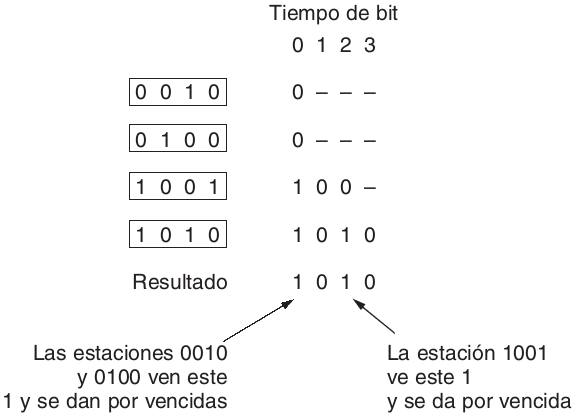
\includegraphics[width=0.5\textwidth-\fboxrule-\fboxrule]{imgs/descendente_binario.png}}}
\end{figure}

\subsubsection{Protocolos de contención limitada}

En condiciones de carga baja, la contención es preferible debido a su bajo retardo. A medida que aumenta la carga, la sobrecarga asociada al arbitraje del canal se vuelve mayor. Lo inverso se cumple para los protocolos libres de colisiones. Con carga baja, tienen un retardo alto, pero a medida que aumenta la carga, mejora la eficiencia del canal en lugar de empeorar.

Se combina entonces la contención y la libertad de colisiones, creando protocolos dinámicos para lograr una buena eficiencia de canal.

Primero dividen las estaciones en grupos (no necesariamente separados). Sólo los miembros del grupo 0 pueden competir por la ranura 0. Si uno de ellos tiene éxito, adquiere el canal y transmite su trama. Si la ranura permanece desocupada o si hay una colisión, los miembros del grupo 1 compiten por la ranura 1, etcétera. 

Se asigna de manera dinámica las estaciones a las ranuras, con muchas estaciones por ranura cuando la carga es baja y pocas estaciones (o incluso sólo una) por ranura cuando la carga es alta.

\subsubsection{WDMA - Protocolos de acceso múltiple por división de longitud de onda}

Para permitir múltiples transmisiones al mismo tiempo, se divide el espectro en canales, y se asignan dos canales a cada estación. Se proporciona un canal estrecho como canal de control para señalizar la estación, y un canal ancho para que la estación pueda enviar tramas de datos.

Cada estación tiene dos emisores y dos receptores, como sigue:
\begin{enumerate}
\item Un receptor de longitud de onda fija para escuchar su propio canal de control.
\item Un emisor sintonizable para enviar por el canal de control de otra estación.
\item Un emisor de longitud de onda fija para la salida de tramas de datos.
\item Un receptor sintonizable para seleccionar al emisor de datos a escuchar.
\end{enumerate}

\subsubsection{Protocolos de LANs inalámbricas}

Tenemos dos problemas a resolver en este tipo de redes:
\begin{description}
\item \textbf{Problema de estación oculta.} Una estación no puede detectar a un competidor potencial por el medio, puesto que dicho competidor está demasiado lejos.
\item \textbf{Problema de estación expuesta.}  Si una estación escucha una transmisión, puede concluir equivocadamente que no puede enviar a su estación destino (para evitar malas recepciones), pero puede que la estación destino está suficientemente lejos de la transmisión detecta y ésta no le hace interferencia.
\end{description}
El problema es que antes de comenzar una transmisión, una estación realmente necesita saber si hay actividad o no alrededor del receptor. 

\begin{description}
\item \textbf{MACA (Acceso Múltiple con Prevención de Colisiones).} El emisor estimula al receptor a enviar una trama corta, de manera que las estaciones cercanas puedan detectar esta transmisión y evitar ellas mismas transmitir durante la siguiente trama de datos. Pasos:
\begin{enumerate}
\item $A$ comienza por enviar una trama corta \textbf{RTS} (\textit{Solicitud de Envío}) a $B$, que contiene la longitud de la trama de datos que seguirá posteriormente. 
\item $B$ contesta con una trama \textbf{CTS} (\textit{Libre para Envío}), que contiene la longitud de los datos (copiada de la trama RTS). Luego $A$ comienza a transmitir.
\item El resto de las estaciones cercanas escuchan al menos uno de los tramos, y se abstienen de transmitir durante un tiempo.
Aún pueden ocurrir colisiones.
\end{enumerate}
En el caso de una colisión, se espera un tiempo aleatorio y se retransmite.
\begin{figure}[ht!]
  \caption{El protocolo MACA. (a) $A$ enviando a $B$ un RTS. (b) $B$ respondiendo a $A$ con un CTS.}
  \label{fig:maca}
  \centerline{\hbox{
   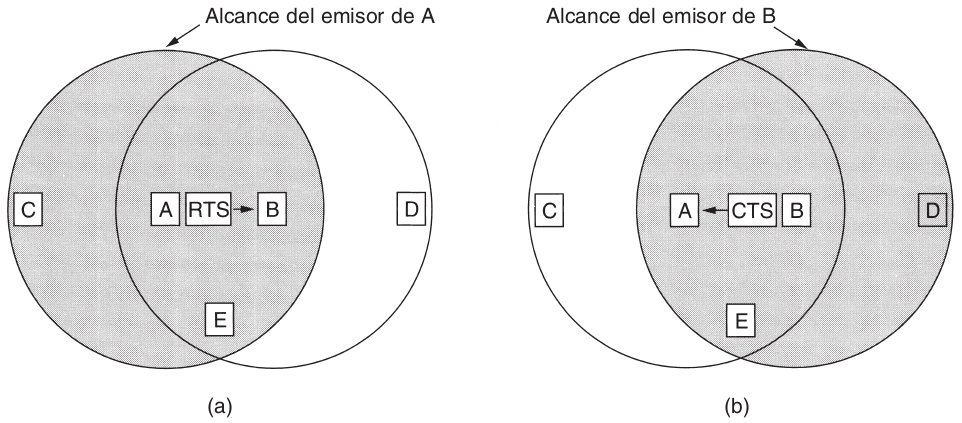
\includegraphics[width=0.85\textwidth-\fboxrule-\fboxrule]{imgs/maca.png}}}
\end{figure}
\item \textbf{MACAW (MACA Inalámbrico)}. Mejora el desempeño del MACA al introducir ACKs (para evitar esperar expirar temporizadores), detección de portadoras (para evitar múltiples RTS), y usar retroceso por cada flujo de datos en vez de por cada estación (mejora equidad).
\end{description}

\subsection{Ethernet}

Todos los sistemas Ethernet usan codificación \textbf{Manchester} debido a su sencillez.

\subsubsection{Cableado Ethernet}

Comúnmente se usan cuatro tipo de cableados (ver Figura \ref{fig:cables_ethernet}):

\begin{figure}[ht!]
  \caption{Los tipos más comunes de cableado Ethernet.}
  \label{fig:cables_ethernet}
  \centerline{\hbox{
   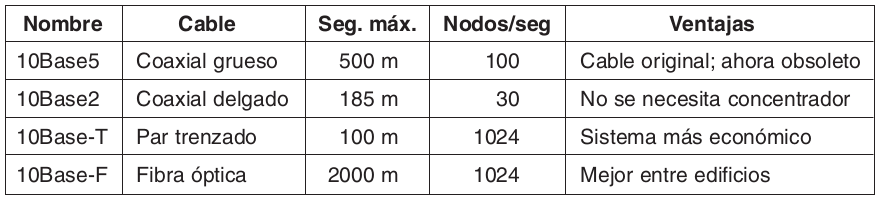
\includegraphics[width=0.85\textwidth-\fboxrule-\fboxrule]{imgs/cables_ethernet.png}}}
\end{figure}

La notación es $X$base$Y$, que significa que opera a $X$ Mbps, que utiliza señalización en la banda base, y que puede manejar segmentos de hasta $Y \cdot 100$ metros.

\begin{description}
\item \textbf{10base5.} Las conexiones se hacen usando \textbf{derivaciones vampiro}, en las que se introduce \textit{cuidadosamente} una punta hasta la mitad del núcleo del cable coaxial. Cable muy rígido.
\item \textbf{10base2.}  Las conexiones forman uniones T. Los conectores son más confiables y sencillos. Cable más flexible, económico y de fácil instalación.
\item \textbf{10base-T.} Todos los cables conducen a un \textbf{concentrador} (\textit{hub}) central, usando pares trenzados, facilitando la detección de errores y el mantenimiento.
\item \textbf{10base-F.} Usa fibra óptica. Es cara debido al costo de los conectores y los terminadores, pero tiene excelente inmunidad contra el ruido y es el método a usar para conexiones entre edificios. Se permiten separaciones de kilómetros entre conexiones. Es más difícil intervenir que una de cobre (más segura).
\end{description}

\begin{figure}[ht!]
  \caption{Tres tipos de cableado Ethernet. (a) 10Base5. (b) 10Base2. (c) 10Base-T.}
  \label{fig:ethernet}
  \centerline{\hbox{
   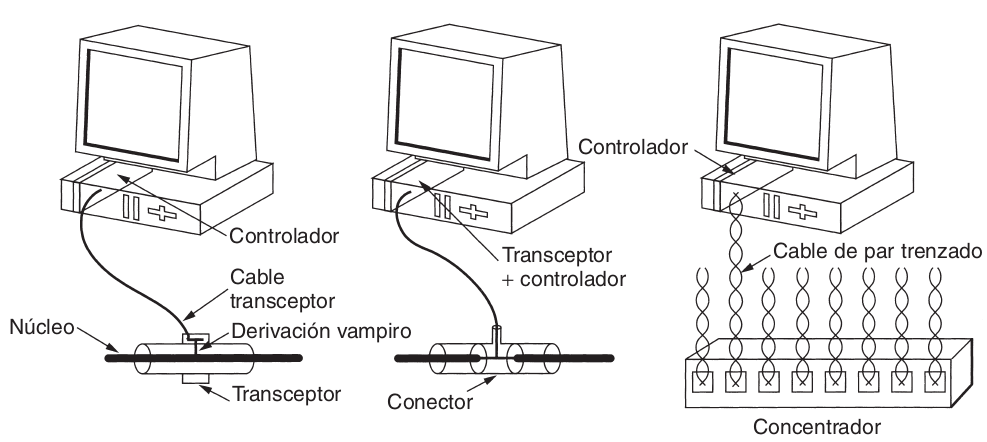
\includegraphics[width=0.9\textwidth-\fboxrule-\fboxrule]{imgs/ethernet.png}}}
\end{figure}

Un \textbf{transceptor} maneja la detección de portadora y de colisiones. Un \textbf{controlador} transmite y recibe tramas de él. Se encarga de ensamblar los datos en el formato de trama adecuado, y de calcular y comprobar el \textit{checksum}.

\subsubsection{El protocolo de subcapa MAC de Ethernet}

\begin{figure}[ht!]
  \caption{Formatos de trama. (a) Ethernet DIX. (b) IEEE 802.3.}
  \label{fig:mac_ethernet}
  \centerline{\hbox{
   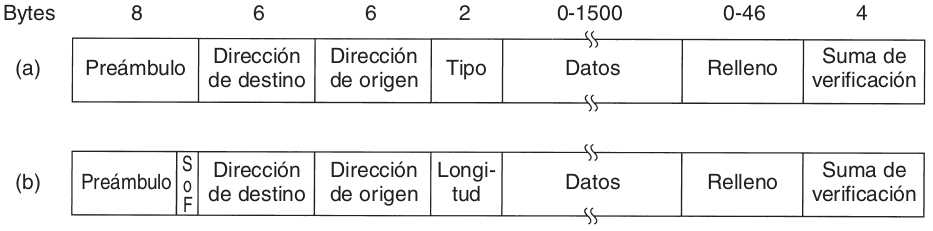
\includegraphics[width=0.85\textwidth-\fboxrule-\fboxrule]{imgs/mac_ethernet.png}}}
\end{figure}

Algunas características de la estructura de trama original de DIX:
\begin{description}
\item \textbf{Preámbulo:} contiene el patrón de bits 10101010. Sirve para sincronizar.
\item \textbf{Dirección de destino:} si empieza con 0, dirección ordinaria; si empieza con 1, dirección de grupo; todos 1, dirección de difusión.
\item \textbf{Tipo:} especifica a qué proceso darle la trama.
\item \textbf{Datos:} tiene una longitud mínima de:
\[\text{Destino + Origen + Tipo + Relleno + \textit{Checksum} = 64 bytes.}\]
Esta longitud mínima es necesaria para evitar que una estación complete la transmisión de una trama corta antes de que el primer bit llegue al extremo más alejado del cable, donde podría tener una colisión con otra trama. \textbf{El tiempo de ida y vuelta de una trama}, a una distancia máxima de 2500 metros y a una velocidad de $2\times 10^8$ m/s, se determina haciendo:
\begin{align*}
\frac{2500}{2\times 10^8}&=12.5 \; [\mu s] &\text{(viaje ida),} \\
12.5 \times 2 &= 25 \; [\mu s] & \text{(ida y vuelta),} \\
25 + 25 &= 50  \; [\mu s] & \text{($25 \; [\mu s]$ de retroceso por repetidores)}.
\end{align*}
A 10 MHz, $50  \; [\mu s]$ se convierten en $500$ [bps], y si lo redondeamos por los 64 bytes a 512[bps], tenemos que el tiempo total de transmisión es de $51.2  \; [\mu s]$. Si aumenta la velocidad, la longitud mínima de la trama debe aumentar o la longitud máxima del cable debe disminuir.
\end{description}

\begin{figure}[ht!]
  \caption{La detección de una colisión puede tardar hasta 2$\tau$.}
  \label{fig:rafaga_ruido}
  \centerline{\hbox{
   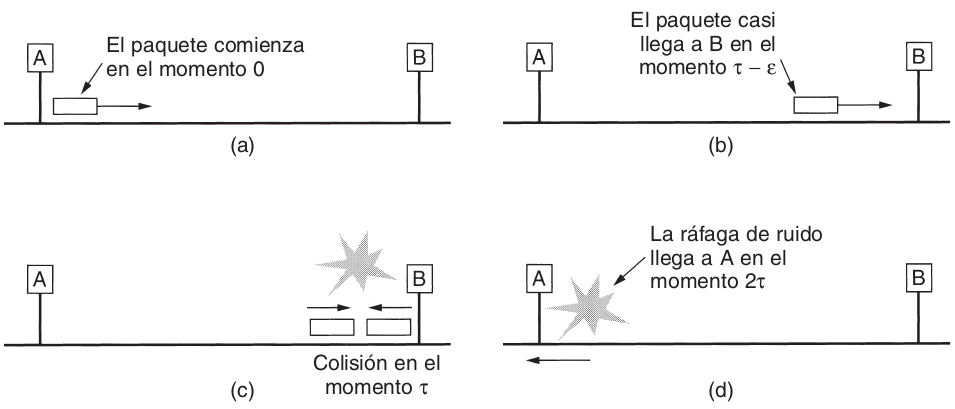
\includegraphics[width=0.85\textwidth-\fboxrule-\fboxrule]{imgs/rafaga_ruido.png}}}
\end{figure}

Los cambios que introdujo el 802.3 fueron:
\begin{itemize}
\item Redujo el preámbulo a 7 bytes, y utilizar el último byte para delimitador de \textit{Inicio de trama}.
\item Cambió el campo \textit{Tipo} por un campo \textit{Longitud} (que marca la longitud de la trama).
\end{itemize}

\subsubsection{Algoritmo de retroceso exponencial binario}

Va cambiando cuanto tiempo esperar luego de una colisión para retransmitir. Cada $i$ colisiones, se escoge un número aleatorio entre 0 y $2^i - 1$, y se salta ese número de ranuras. Sin embargo, tras haberse alcanzado 10 colisiones, el intervalo de aleatorización se congela en un máximo de 1023 ranuras. Tras 16 colisiones, el controlador informa de un fracaso a la computadora. La recuperación posterior es responsabilidad de las capas superiores.

Asegura retardo pequeño con pocas estaciones, resolución razonable con muchas estaciones.

\subsubsection{Ethernet conmutada}

En algún momento, la LAN se saturará al aumentar el tráfico. Una ethernet conmutada trata de forma diferente con el aumento de carga, usando como base un \textbf{conmutador} (\textit{switch})\footnote{Contiene una matriz de conmutación de alta velocidad y espacio para 4 a 32 tarjetas de línea, cada una de las cuales contiene de uno a ocho conectores de par trenzado a un \textit{host}.}.

\begin{figure}[ht!]
  \caption{Ejemplo sencillo de Ethernet conmutada.}
  \label{fig:conmutada}
  \centerline{\hbox{
   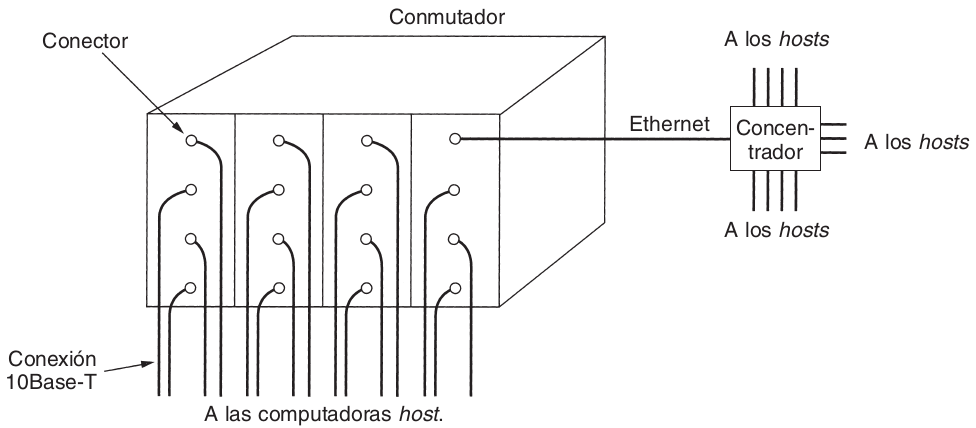
\includegraphics[width=0.85\textwidth-\fboxrule-\fboxrule]{imgs/conmutada.png}}}
\end{figure}

Cuando una estación quiere transmitir, envía una trama estándar al conmutador. La tarjeta que recibe la trama la revisa para ver si está destinada a una de las otras estaciones conectadas a la misma tarjeta. De ser así, la trama se copia ahí. Si no, la trama se envía a través de la matriz de conmutación de alta velocidad a la tarjeta de la estación de destino.

¿\textit{Qué ocurre si dos máquinas conectadas a la misma tarjeta de conexión transmiten tramas al mismo tiempo}? Depende de como esté la tarjeta construida:
\begin{description}
\item \textbf{LAN local dentro de la tarjeta.} Se comporta como una CSMA/CD con retroceso exponencial binario. Sólo una transmisión por tarjeta en cada instante es posible. Cada tarjeta forma su propio \textbf{\textbf{dominio de colisión}}, independientemente de las demás. Las colisiones son imposibles y el desempeño mejora.
\item \textbf{Almacenamiento en RAM con búfer.} Cada trama se almacena en el búfer de su puerto. Permite recibir y transmitir múltiples tramas al mismo tiempo, formando un dúplex. Cada puerto es un dominio de colisión independiente, por lo que no ocurren colisiones. Algunos puertos pueden usarse como conmutadores.
\end{description}

\subsubsection{Fast Ethernet}

El comité 802.3 decidió crear una Ethernet mejorada (y no completamente nueva, sino optimizando la anterior), que pasaría a llamarse \textbf{802.3u}, por tres razones principales:
\begin{enumerate}
\item La necesidad de compatibilidad hacia atrás con las LANs Ethernet existentes.
\item El miedo de que un nuevo protocolo tuviera problemas no previstos.
\item El deseo de terminar el trabajo antes de que la tecnología cambiara.
\end{enumerate}

\begin{figure}[ht!]
  \caption{El cableado original de Fast Ethernet.}
  \label{fig:fast_ethernet}
  \centerline{\hbox{
   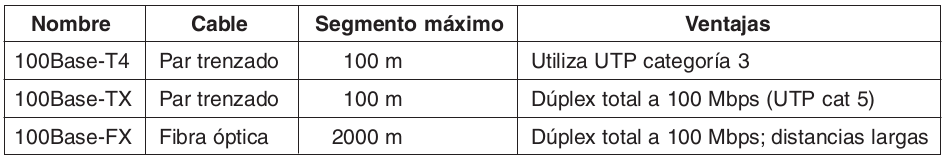
\includegraphics[width=0.85\textwidth-\fboxrule-\fboxrule]{imgs/fast_ethernet.png}}}
\end{figure}


\subsubsection{Gigabit Ethernet}

Los objetivos del comité \textbf{802.3z} eran esencialmente los mismos que los del comité 802.3u: hacer que Ethernet fuera 10 veces más rápida y que permaneciera compatible hacia atrás con todos los estándares Ethernet existentes. Todas las configuraciones de Gigabit Ethernet son de punto a punto en lugar de múltiples derivaciones como en el estándar original.

\begin{figure}[ht!]
  \caption{(a) Ethernet de dos estaciones. (b) Ethernet con múltiples estaciones.}
  \label{fig:gigabit}
  \centerline{\hbox{
   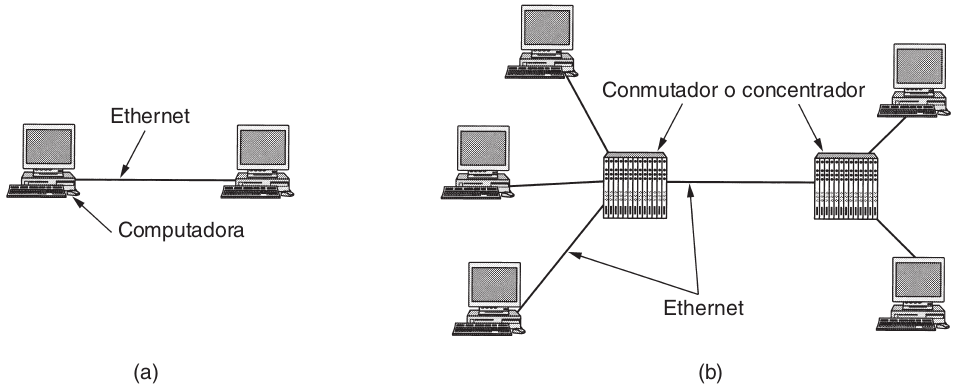
\includegraphics[width=0.85\textwidth-\fboxrule-\fboxrule]{imgs/gigabit.png}}}
\end{figure}

Gigabit Ethernet soporta dos modos diferentes de funcionamiento: 
\begin{description}
\item \textbf{Dúplex total:} modo ``normal'', el cual permite tráfico en ambas direcciones al mismo tiempo. Se utiliza cuando hay un conmutador central conectado a computadoras (o a otros conmutadores) en el periférico. 
\item \textbf{Semi-dúplex:} se utiliza cuando las computadoras están conectadas a un concentrador en lugar de a un conmutador.
\end{description}

\begin{figure}[ht!]
  \caption{Cableado de Gigabit Ethernet.}
  \label{fig:cableado_gigabit}
  \centerline{\hbox{
   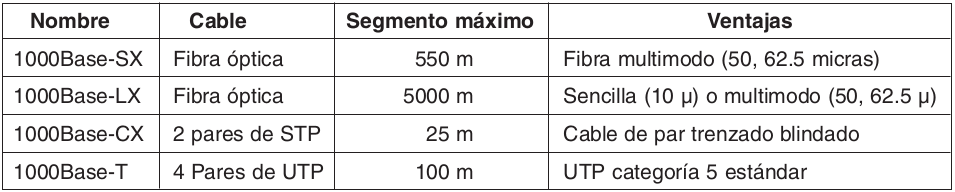
\includegraphics[width=0.85\textwidth-\fboxrule-\fboxrule]{imgs/cableado_gigabit.png}}}
\end{figure}

\subsubsection{Estándar IEEE 802.2: control lógico del enlace}

Hay sistemas en los que se desea un protocolo de enlace de datos con control de errores y control de flujo. El protocolo \textbf{LLC} (\textbf{Control Lógico del Enlace}), esconde las diferencias entre los distintos tipos de redes 802, proporcionando un formato único y una interfaz con la capa de red.

La capa de red de la máquina emisora pasa un paquete al LLC usando las primitivas de acceso del LLC. A continuación, la subcapa LLC agrega un encabezado LLC que contiene los números de secuencia y confirmación de recepción. La estructura resultante se introduce entonces en el campo de carga útil de una trama 802 y se transmite. En el receptor ocurre el proceso inverso.

\begin{figure}[ht!]
  \caption{(a) Posición del LLC. (b) Formatos de protocolo.}
  \label{fig:llc}
  \centerline{\hbox{
   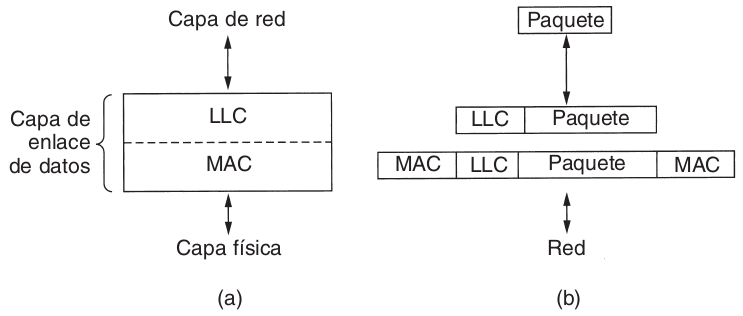
\includegraphics[width=0.65\textwidth-\fboxrule-\fboxrule]{imgs/llc.png}}}
\end{figure}

El LLC proporciona tres opciones de servicio: servicio no confiable de datagramas, servicio de datagramas sin confirmación de recepción y servicio confiable orientado a la conexión. El encabezado LLC contiene tres campos: 
\begin{description}
\item \textbf{Punto de acceso de destino.} Indica de cuál proceso proviene la trama.
\item \textbf{Punto de acceso de origen.} Indica a dónde se va a enviar.
\item \textbf{Campo de control.} Contiene números de secuencia y de confirmación de recepción. Se utilizan principalmente cuando se necesita una conexión confiable en el nivel de enlace de datos.
\end{description}

\subsubsection{Retrospectiva de Ethernet}

La razón principal de su longevidad es su simpleza y flexibilidad, que se traduce en la práctica como confiable, barato y fácil de mantener. Además, interactúa fácilmente con TCP/IP.

\subsection{LANs inalámbricas (VLANs)}

Pueden funcionar con o sin estación base.

\begin{figure}[ht!]
  \caption{Parte de la pila de protocolos del 802.11.}
  \label{fig:protocolos_802}
  \centerline{\hbox{
   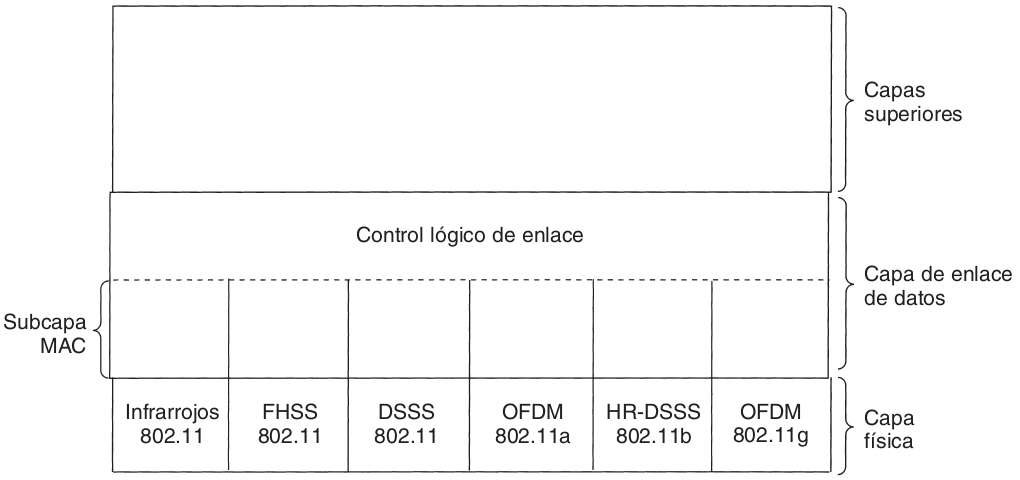
\includegraphics[width=0.85\textwidth-\fboxrule-\fboxrule]{imgs/protocolos_802.png}}}
\end{figure}

\subsubsection{La capa física del 802.11}

\begin{description}
\item \textbf{Infrarrojos:} 
\begin{itemize}
\item Utiliza transmisión difusa (no requiere línea visual).
\item Se permiten dos velocidades: 1 y 2 Mbps.
\item No puede penetrar paredes, por lo que trabaja en celdas aisladas.
\end{itemize}
\item \textbf{FHSS (Espectro Disperso con Salto de Frecuencia):}
\begin{itemize}
\item Utiliza 79 canales de 1 MHz cada uno.
\item Utiliza un generador pseudo-aleatorio (más \textit{seguridad}) de números para crear la secuencia a saltar de frecuencias.
\item \textbf{Tiempo de permanencia} en cada frecuencia debe ser $<400$ mseg.
\item Insensible a la interferencia.
\item Bajo ancho de banda.
\end{itemize}
\item \textbf{DSSS (Espectro Disperso de Secuencia Discreta):}
\begin{itemize}
\item Restringido a 1 o 2 Mbps.
\item Similitudes con el CDMA, pero usa \textbf{secuencia Barker}.
\item Utiliza modulación por desplazamiento de fase a 1 Mbaudio.
\end{itemize}
\item \textbf{OFDM (Multiplexación por División de Frecuencias Ortogonales) [802.11a]:}
\begin{itemize}
\item Envía hasta 54Mbps en banda ancha de 5 GHz.
\item Utiliza 52 frecuencias diferentes: 48 para datos y 4 para sincronización.
\item Mejor inmunidad a la interferencia de bandas estrechas.
\item Buena inmunidad al desvanecimiento de mútiples rutas.
\end{itemize}
\item \textbf{HR-DSSS (DSSS de Alta Velocidad) [802.11b]:}
\begin{itemize}
\item 11 Mbps en la banda de 2.4 GHz.
\item Las tasas sde datos soportodas son de 1, 2, 5.5, y 11 Mbps. Las dos primeras usan PSK y las dos más rapidas usan códigos \textbf{Walsh/Hadamard}.
\end{itemize}
\item \textbf{802.11g:}
\begin{itemize}
\item Versión mejorada de la 802.11b.
\item Utiliza OFDM en la banda 2.4 GHz.
\item Límite teórico de 54 Mbps.
\end{itemize}
\end{description}

\subsubsection{El protocolo de la subcapa MAC del 802.11}

Existen los problemas de estaciones ocultas/expuestas. Además, la mayoría de las radios son semidúplex, lo que significa que no pueden transmitir y escuchar ráfagas de ruido al mismo tiempo en una sola frecuencia. Por ello no utiliza CSMA/CD (como Ethernet).

Para sobreponerlo, se soportan diferentes modos de funcionamiento:
\begin{description}
\item \textbf{DFC (Función de Coordinación Distribuida):} no utiliza ningún tipo de control central.
\item \textbf{PCF (Función de Coordinación Puntual):} utiliza la estación base para controlar toda la actividad en su celda.
\item \textbf{Combinación de ambos (DFC y PCF).}
\end{description}

% Me falta todo desde aca hasta la 4.4.4, quedara para final

\subsubsection{La estructura de trama 802.11}

Define tres clases diferentes de tramas en el cable: de datos, de control y de administración. 

\begin{figure}[ht!]
  \caption{La trama de datos 802.11.}
  \label{fig:trama_80211}
  \centerline{\hbox{
   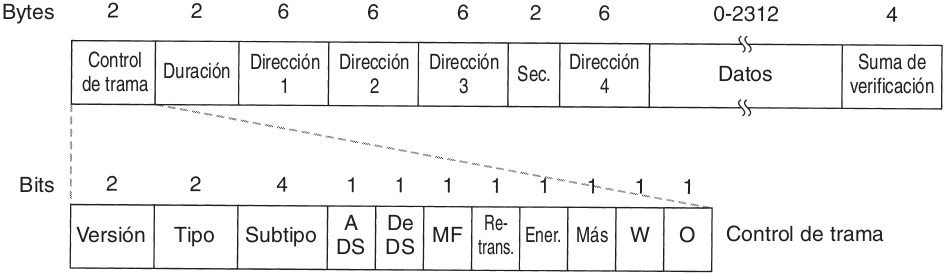
\includegraphics[width=0.95\textwidth-\fboxrule-\fboxrule]{imgs/trama_80211.png}}}
\end{figure}

El formato de la trama de datos está dado por:
\begin{enumerate}
\item \textbf{Control de trama.} Está compuesto de 11 subcampos:
\begin{itemize}
\item \textit{Versión del protocolo:} permite varias versiones al mismo tiempo en una misma celda.
\item \textit{Tipo:} de datos, control o de administración.
\item \textit{Subptipo:} RTS o CTS por ejemplo.
\item \textit{A DS:} va hacia el sistema de distribución entre celdas.
\item \textit{De DS:} viene del sistema de distribución entre celdas.
\item \textit{MF:} ``\textit{more fragments}'', vienen más fragmentos.
\item \textit{Retransmisión:} marca una retransmisión de una trama.
\item \textit{Administración de energía:} pone o saca al receptor del estado de hibernación.
\item \textit{Más:} tramas adicionales por entregar.
\item \textit{W:} se usó WEP (Privacidad Inalámbrica Equivalente).
\item \textit{O:} las tramas vienen ordenadas.
\end{itemize}
\item \textbf{Duración.} Indica cuánto tiempo ocuparán el canal la trama y ACK.
\item \textbf{Direcciones.} Dos para el destino y para el origen, y otras dos para la estaciones base de origen y destino para el tráfico entre celdas.
\item \textbf{Secuencia.} Permite que se numeren los fragmentos.
\item \textbf{Datos.} La carga útil.
\item \textbf{Checksum.}
\end{enumerate}

Las tramas de administración tienen un formato similar, excepto que no tienen una de las direcciones de la estación base porque se restringen a una celda. Las tramas de control son más cortas, tienen una o dos drecciones, y no tienen \textit{Datos} ni \textit{Secuencia}. Lo importante es el \textit{Subtipo}.

\subsubsection{Servicios}

Cada LAN inalámbrica debe proporcionar nueve servicios: cinco servicios de \textbf{distribución} y cuatro de \textbf{estación}. Los servicios de \textit{distribución} se relacionan con la administración de membresías dentro de la celda y con la interacción con estaciones que están fuera de la celda. En contraste, los servicios de \textit{estación} se relacionan con la actividad dentro de una sola celda.
\\

\underline{\textbf{Servicios de distribución:}}
\begin{enumerate}
\item \textbf{Asociación.} Conecta estaciones móviles con estaciones base.
\item \textbf{Disociación.} Rompe relaciones de estaciones.
\item \textbf{Reasociación.} Cambia estación base preferida de una estación.
\item \textbf{Distribución.} Determina enrutamiento de tramas.
\item \textbf{Integración.} Maneja la traducción.
\end{enumerate}

\underline{\textbf{Servicios de estación:}}
\begin{enumerate}
\item \textbf{Autenticación.} Primero debe autentificarse una estación para permitírsele enviar datos.
\item \textbf{Desautenticación.} ¿Abandona la red? $\Rightarrow$ Se desautentica.
\item \textbf{Privacidad.} Maneja la codificación/decodificación.
\item \textbf{Entrega de datos.} Las capas superiores deben tratar con detección y corrección de errores.
\end{enumerate}

\setcounter{subsection}{6}
\subsection{Conmutación en la Capa de Enlace de Datos}

Muchas organizaciones tienen varias LANs y desean interconectarlas. Esto se realiza mediante \textbf{puentes}. Hay seis razones por lo que se podría contar con muchas LANs en una organización:
\begin{enumerate}
\item Debido a la autonomía de sus dueños (metas distintas).
\item Es \textbf{más económico} tener LANs dispersas y conectadas mediante puentes, que una sola gran LAN.
\item Puede ser necesario dividir una LAN en varias LANs individuales para manejar la carga.
\item Con puentes entre LANs, puede \textbf{aumentar la distancia física total cubierta}.
\item Es \textbf{más confiable}: en una gran LAN, un sólo nodo defectuoso afecta toda la red. Al agregar puentes en lugares críticos, se detiene la propagación de errores.
\item Es \textbf{más seguro}: es posible aislar partes de la red para evitar que tráfico delicado llegue a estaciones indeseadas.
\end{enumerate}

Un puente que conecta $k$ LANs diferentes tendrá $k$ subcapas MAC y $k$ capas físicas distintas, una para cada tipo.

\subsubsection{Problemas de construir puertos entre 802.3, 802.11, y 802.16}

\begin{enumerate}
\item Cada LAN utiliza un \textbf{formato de trama distinto}. Se requiere reformatear cada trama entre los puentes de LANs distintas, lo que conlleva recursos de CPU.
\item Entre las LANs puede haber \textbf{diferencias} en la \textbf{tasa de datos}.
\item Las distintas LANs tienen \textbf{distintas longitudes máximas de trama}, por lo que se requiere descartar tramas muy grandes.
\item Ethernet no tiene \textbf{calidad del servicio} ni no soporta \textbf{encriptación} en la CdE, por lo que ambas se pierden al pasar tráfico por Ethernet.
\end{enumerate}

\subsubsection{Interconectividad local}

Los \textit{puentes} no deberían afectar de ninguna manera el funcionamiento de una LAN existente: deberían ser \textbf{transparentes}. Para ello, se requiere que:
\begin{itemize}
\item Trabajar en modo \textbf{promiscuo} \footnote{Acepta todas las tramas transmitidas sobre las LANs a las cuales está conectado.}.
\item Armar una tabla de \textit{hash} en su interior utilizando el algoritmo de \textbf{inundación} \footnote{Todas las tramas que llegan al puente con un destino desconocido se envían a todos los destinos desconocidos (excepto de los cuales provino), hasta aprender la dirección de estos destinos desconocidos (usando el algoritmo de \textbf{aprendizaje hacia atrás}).}.
\item Para manejar topologías dinámicas, siempre que se realiza una entrada en una tabla \textit{hash} se le asocia también la hora de llegada de la trama. Periódicamente, se analiza la tabla de \textit{hash} y se purga las entradas que tengan más de algunos minutos, para mantener las direcciones actualizadas.
\item El procesamiento de enrutamiento para una trama entrante depende de:
\begin{enumerate}
\item LAN destino $=$ LAN origen $\Rightarrow$ \textbf{descartar} la trama.
\item LAN destino $\neq$ LAN origen $\Rightarrow$ \textbf{reenviar} la trama.
\item LAN destino desconocida $\Rightarrow$ \textbf{inundación}.
\end{enumerate}
Este algoritmo debe aplicarse cada vez que llega una trama.
\end{itemize}

\subsubsection{Puentes con árbol de expansión}

Para incrementar la \textbf{confiabilidad}, se pueden usar dos o más puentes en paralelo entre pares de LANs. Sin embargo, este arreglo genera problemas adicionales porque produce ciclos en la topología: durante la \textbf{inundación}, se satura la red y no se resuelven las direcciones.

La solución es utilizar un \textbf{árbol de expansión}, que es acíclico y estable una única ruta de un nodo a otro. Abarca todas las LANs, pero puede no incluir a todos los puentes (para evitar ciclos).

Para construirlo, se elige un puente como raíz, y se calculan las rutas más cortas a todas las LANs y puentes. Si un puente o una LAN falla, se recalcula un nuevo árbol. El algoritmo persiste operando para detectar cambios en la topología y actualizar el árbol.
\vfill

\pagebreak
\section{Anexo}

\subsection{Dispositivos Físicos}
A continuación una breve descripción de cada uno de ellos y, entre paréntesis, en que capa trabajan.
\begin{description}
\item \textbf{Repetidores} (CF). Dispositivos análogos conectados a dos segmentos de cable. Una señal que aparece en uno de ellos es amplificada y enviada al otro. Trabajan con señales, ignorando a las tramas, paquetes o encabezados.
\item \textbf{Concentradores} (CF). Tiene numerosos puertos de entrada que une de manera eléctrica. Reenvía (sin amplificar) todas las tramas a todas las salidas. Es un sólo dominio de colisión: las tramas que llegan juntas, colisionan.
\item \textbf{Puentes} (CED). Examinan las direcciones de la CED para enrutar los datos. Reciben una trama, verifican la dirección de origen, y comprobando su tabla de \textit{hash}, la reenvía por el puerto adecuado. Cada puerto es un dominio de colisión.
\item \textbf{Conmutadores} (CED). Similares a los puentes, pero conectan \textit{hosts}. Poseen búferes en cada puerto, por lo que nunca pierden tramas por colisiones (a excepeción de que las tramas lleguen a más velocidad de la que se transmiten, reduciendo el espacio de búfer).
\item \textbf{Enrutadores} (CdR). Examinan las direcciones de los paquetes y realizan su trabajo de enrutamiento con base a ellas. Eliminan el encabezado y terminador de trama.
\item \textbf{Puertas de Enlace de Transporte} (CT). Conectan dos computadoras con diferentes protocolos de transporte orientados a la conexión.
\item \textbf{Puertas de Enlace de Aplicación} (CA). Comprenden el formato y contenido de los datos y traducen los mensajes de un formato a otro.
\end{description}
\vspace{0.5cm}
\begin{figure}[ht!]
  \caption{(a) Los dispositivos y sus capas correspondientes. (b) Tramas, paquetes y encabezados.}
  \label{fig:dispositivos}
  \centerline{\hbox{
   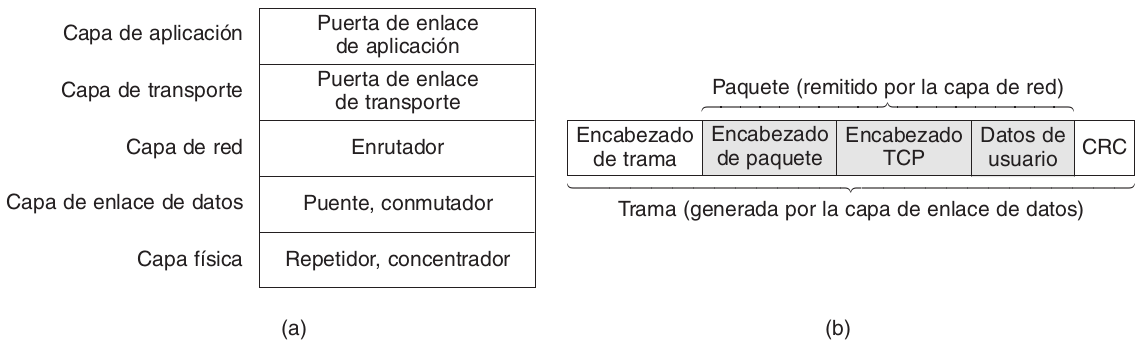
\includegraphics[width=\textwidth-\fboxrule-\fboxrule]{imgs/dispositivos.png}}}
\end{figure}

\begin{figure}[ht!]
  \caption{Acceso a un servidor Web a través de una conexión remota.}
  \label{fig:old}
  \centerline{\hbox{
   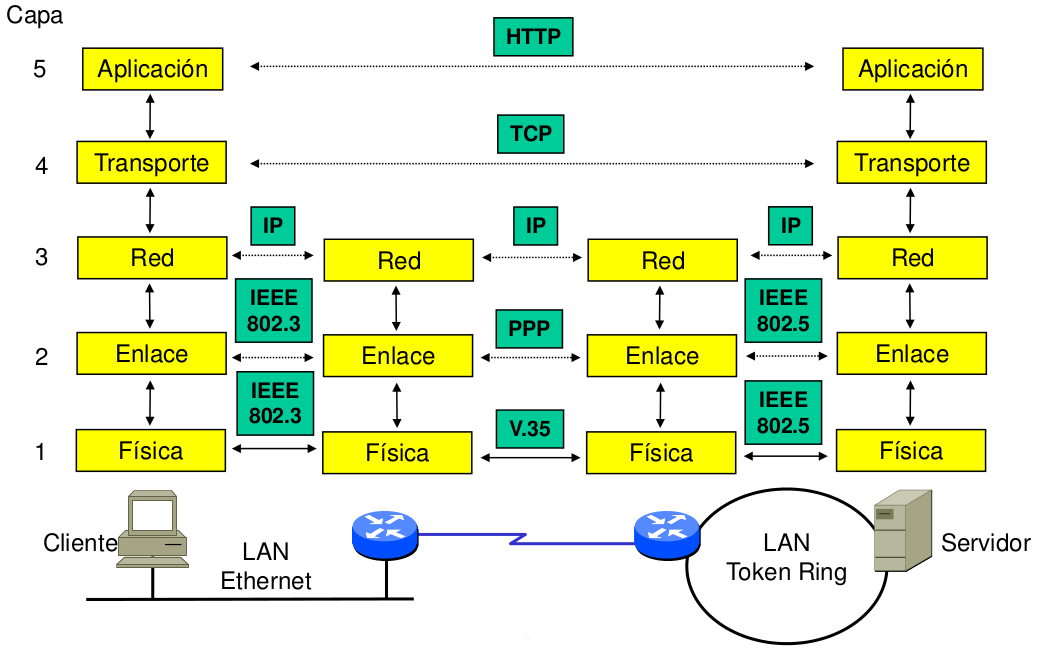
\includegraphics[width=0.85\textwidth-\fboxrule-\fboxrule]{imgs/old.png}}}
\end{figure}


\pagebreak
\subsection{Parciales}

\subsubsection{Parcial I (2011)}
\begin{enumerate}
\item Realizar un diagrama de capas OSI para 2 Host y un Router. Especificar protocolos y transferencias de datos.
\item Capa de enlace de OSI. Explicar funciones.
\item Problemas de transmisión en una comunicación. Nombrarlos y explicarlos brevemente.
\item Explicar ruido térmico y cómo se calcula.
\item ¿En qué consiste PSK?
\item Códigos de Aleatorización. Para qué se usan?. Nombrar 2.
\item Nyquist y Shannon y la relación entre ellos.
\item Realizar un diagrama de fases para 64QAM.
\item Tabla comparativa en medios guiados.
\item Enlace de microondas. Qué consideraciones hay que tener?
\end{enumerate}

\subsubsection{Recuperatorio Parcial I (2011)}
\begin{enumerate}
\item Realizar diagrama de capas de TCP/IP con dos hosts y un router.
\item Definir los tipos de ruido y explicar uno de ellos.
\item Realizar un diagrama de fases 16PSK.
\item Definir las primitivas de modulacion analogica (solamente ASK,PSK,FSK, no MFSK, BFSK, etc.).
\item Explicar como funciona QAM.
\item Explicar un metodo de sustitucion detalladamente (son las tecnicas de aleatorizacion).
\item Explicar como funciona la transmision por fibra optica.
\item Que hay que tener en cuenta para la transmision por microondas. Demostrar con formulas matematicas.
\item Realizar un grafico del espectro electromagnetico de $10^2$ hasta $10^11$ Hz (o MHz, no recuerdo) y nombrar que sistemas de transmision incluyen (algo asi era la pregunta, no me acuerdo exactamente porq ni la sabia).
\end{enumerate}

\subsubsection{Parcial II}
\begin{enumerate}
\item Explicar las alternativas para delimitar las tramas.
\item Explique el concepto de ventana corrediza. Ejemplifique con un gráfico el concepto de ventana corrediza de tamaño 1 y número de secuencia de 3 bits.
\item Describa el formato de la trama HDLC y explique sus campos.
\item Describa el diagrama de fase simplificado para activar y desactivar una linea PPP. En el mismo, detalle cuando estamos en presencia de LCP y cuando en presencia de NCP.
\item Explique como se calcula el tiempo 2 $\tau$ (dos tau) en las redes IEEE802.3.
\end{enumerate}

\subsection{Finales}
\subsubsection{Examen Segundo Turno Diciembre 2011}
\begin{enumerate}
\item Codificación de señales.
\subitem Haga un grafico de cada una de las primitivas de codificación (Unipolar, Polar, Bipolar). Ventajas y desventajas.
\item Medio Fisico: Radio Frecuencia.
\subitem Explique que son las microondas. Describa las ecuaciones del calculo del enlace, tanto para distancia como para 
potencia
\item Medio Fisico: Fibra Optica.
\subitem Explique como funciona la fibra optica y sus clasificaciones. Demuestre el calculo de la apertura numerica y que 
significa este concepto
\item Capa de Enlace.
\subitem Describa el protocolo HDLC. Su trama, su funcionamiento, en que ocasiones se usa y algun dato que quiera 
agregar
\item 802.11. Subcapa MAC.
\subitem Explique el funcionamiento de la subcapa MAC de 802.11
\end{enumerate}
\end{document}